\chapter{Establishment of a culture model for network activity in neuronal ensembles}
\label{chap:activity}
    \section{Introduction}
     As reviewed in section \ref{sec:introduction:MEANetwork}, neuronal cultures grown on multi electrode arrays have emerged as a successful model for studying generic properties of neuronal ensembles at the network level. The overall purpose of this Ph.D work is to provide this model system with an added functionality of phasic volume transmission, thus achieving a novel experimental platform for studying how fine temporal feature of extrasynaptic agonist transients interact with the activity. In this first chapter we describe the establishment of standard neuronal cultures on MEA model system based on embryonic mouse tissue within our laboratory group. We followed their development for over 3 weeks \textit{in vitro} and demonstrated that they develop normally and exhibit hallmark network activity, both spontaneous and evoked, and comply with the characteristics reported in previous work \cite{chiappalone2006dissociated,wagenaar2006extremely,van2004longterm,breskin2006percolation,penn2016network}. To date, MEA investigation have been dominated by use of primary cultures derived from rat. However, mouse is generally a more popular neuroscience model and offers a far greater library of molecular and genetic tools so using it as a tissue source might be beneficial. Thus, the data provided here is useful in the sense that it establishes the compatibility of mouse cultures with the MEA technique and allows comparison of their activity traits to what has been observed in rat preparations.

     As a next step, prior to engaging in the development of the microfluidics system for rapid pulsing, we wanted to explore whether useful neuromodulator functionality may be generated simply through bath application, i.e., by manually pipetting the agonist onto the culture and then washing it away by replacement of the media. We used this approach to revisit the long standing issue of plasticity in these systems. Synaptic plasticity without neuromodulation in neuronal cultures on MEA has been controversial as multiple reports produced contradictory or negative results (reviewed further in section \ref{sec:activity:plasticityProtocol}) and it has been suggested that the lack of neuromodulatory control is partly responsible for the inability to generate this functionality. Thus, as a final step in this chapter, we revisited the question of plasticity induction with and without bath applied dopamine. As will be shown in section \ref{sec:activity:plasticityProtocol}, these experiments produced ambiguous results because the effect of the media replacement cannot be easily separated from that of the dopamine, hence confusing the interpretation. This study thus serves to provide motivation for the development of the microfluidics technology in the following chapters.

     We conclude the chapter by reporting on a pilot study examining rat based preparation and comparing their activity measures to the mouse data. The reason for this is that even though the mouse cultures were ultimately shown to be useful, they exhibited pronouncedly slower and delayed synaptic development as compared to rat cultures and they were much harder to culture on the MEA surface (i.e., a high proportion of the seeded cultures did not develop at all). Consequently, since the tissue source is not critical in the context of this Ph.D, we finally decided to use rat preparations in the remainder of the work.
        	
    \section{Development of spontaneous activity in Mouse cultures}
    \label{sec:activity:spontActivity}
    Primary mouse embryonic cortical cultures were seeded on pre-coated MEAs as described in sections \ref{sec:methods:surface} and \ref{sec:methods:culture}. All MEAs used for the work undertaken in this chapter are of \(8\times8\) configuration with \(30 \mu m\) electrodes and \(200 \mu m\) electrode spacing (see section \ref{sec:methods:MEARecording}).

    Figure \ref{fig:activity:mouseImages} A-C shows microscope images of a representative culture over 3 weeks in culture. The images show how over the first few days the cells extended neurites and dendrites. In later days of development, the gaps between the cells seem to fill up with tissue, presumably neurites and ECM. In the case of these mouse cultures, many of the preparations did not develop properly whereby, despite good initial adhesion, the majority of the plated cells did not continue differentiating and after a few days detached from the surface and degenerated (figure \ref{fig:activity:mouseImages} D). This was the case for over half of plated cultures and these were discarded from the experiment. Cultures prepared from rat embryos (discussed at the end of this chapter) did not present this sort of inconsistency and generally developed at a high success rate despite using the same MEAs and generally same coating and seeding procedures (sections \ref{sec:methods:surface} and \ref{sec:methods:culture}).
       \begin{figure}[!htb]
            \centering
            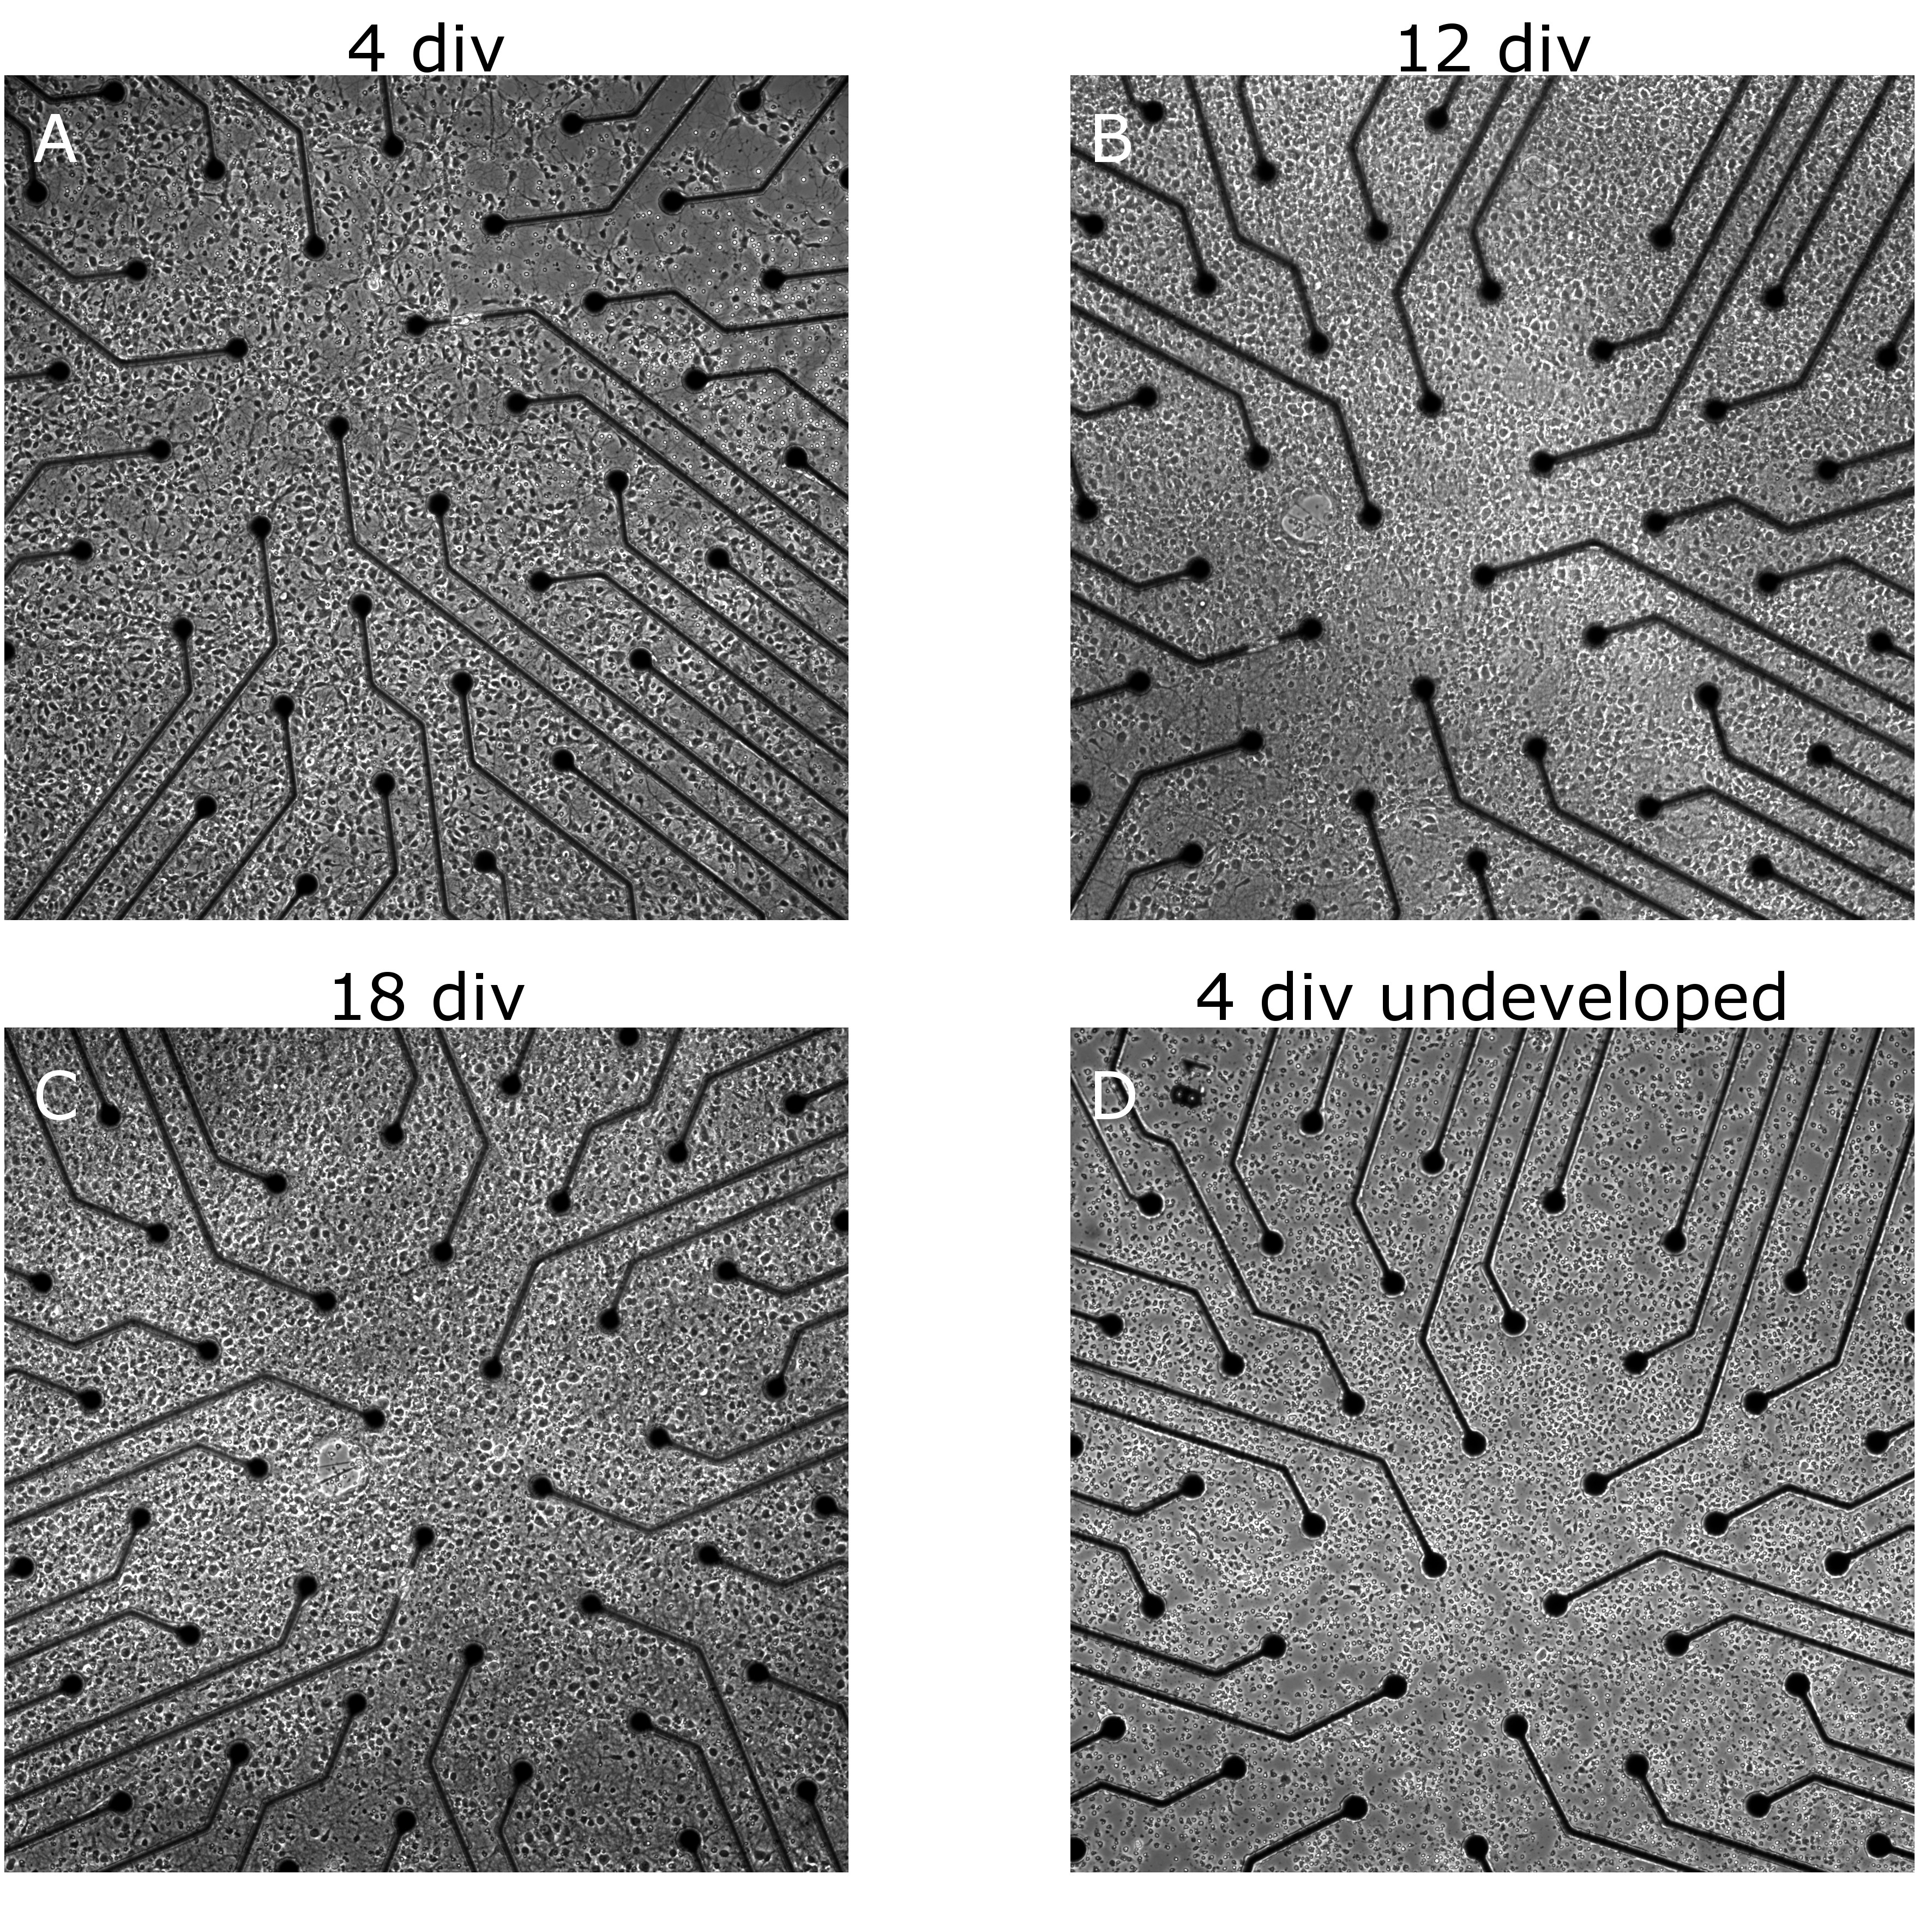
\includegraphics[width=15cm]{chapter3/figures/mouseImages/mouseImages.jpg}

            \caption[Representative images of a cortical mouse culture developing on a planar multi electrode array]{\textbf{Cortical mouse cultures develop to become a densely interconnected neural tissue.} (A) Cortical culture prepared from mice embryos, plated on micro-electrode arrays and imaged at 4 days in vitro. Arrowheads point to culture areas devoid of cell bodies where extending neurites may be observed. (B) Same location in the culture shown in panel A imaged at 16 days in vitro. At this point, individual neurites could not be observed even in areas no harboured by cell bodies (arrowheads), possibly due to the density of the neuritic mass or to engulfment by ECM. (C) The culture shown in panels A-B imaged in lower magnification for reference. (D) Example of a seeded culture that did not show proper development. In such cases, the seeded cells remained mostly circular indicating a lack of surface adhesion and little or no neurites were observed between the cell bodies (compare with A). The electrodes were \(30 \mu m\) wide and spaced \(200 \mu m\) apart.}
            \label{fig:activity:mouseImages}
        \end{figure}




    We monitored the spiking activity of the mouse cultures for 3 weeks in \textit{in vitro}. The analysis performed throughout this thesis is restricted solely to spiking activity and lower frequencies associated with local field potentials were filtered out of the data. Spike detection was preformed through a combination of match filtering and simple threshold crossing. A second pre-analysis step detected and removed erroneous spike waveforms induced by electromagnetic noise and which generated synchronized spiking artefacts across several channels (see section \ref{sec:methods:MEARecording} for full description of the pre-analysis). No spike sorting was attempted as this has been shown to be ineffective in culture \cite{herzog2011optical}.

        \begin{figure}[!htb]
            \centering
            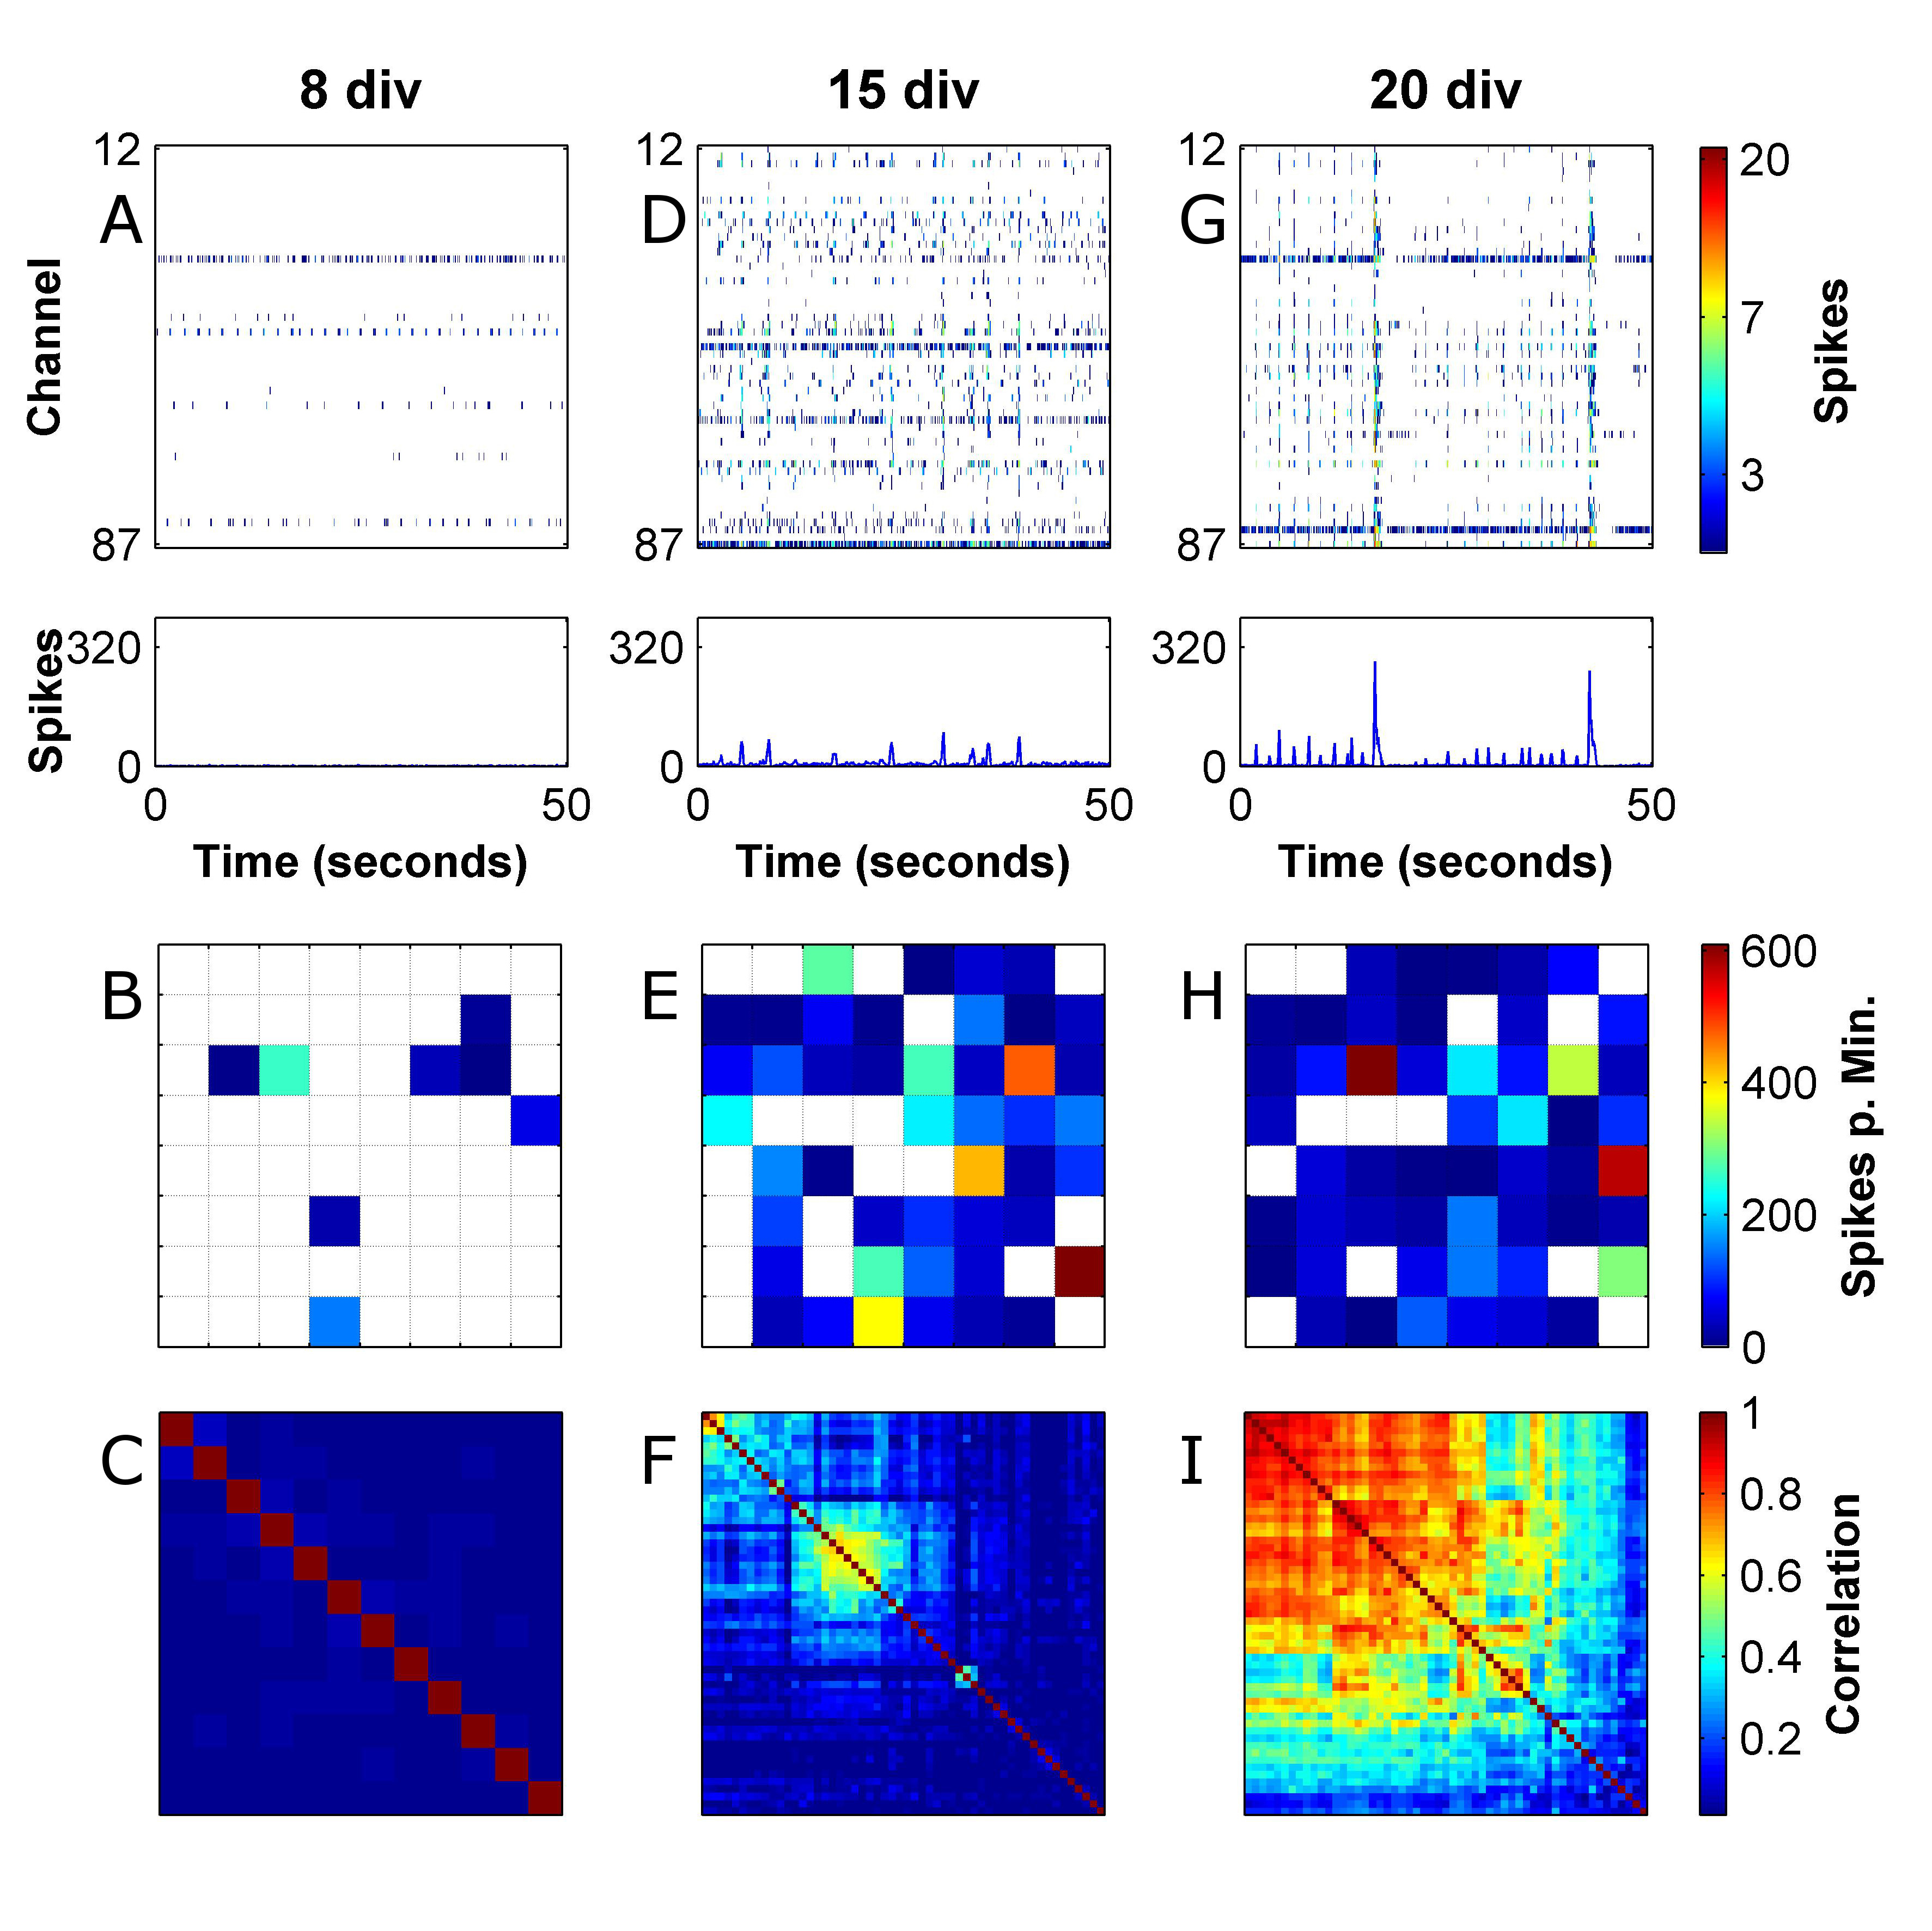
\includegraphics[width=15cm]{chapter3/figures/devExample/devActivity.jpg}

            \caption[Development of synchrony in the spontaneous activity of a representative mouse culture]{\textbf{Spontaneous activity in mouse culture develops from tonic firing into synchronized bursting events.} (A,D,G) Raster plot of spontaneous activity in mouse culture in 3 developmental time points exhibiting the change in the activity structure. Over development, network spiking activity gradually spread to most of the channels and became organized in network bursts. Raster plots are presented in \(100 ms\) bins. Bottom panels show sum of all channels. (B,E,H) Activity maps showing the spatial organization of activity on the MEA in the same time points. (C,F,I) Dendrogram- sorted correlation matrices showing groupings of channels into correlated blocks. Development of synchronization was manifested as blocks of correlated channel in the correlation matrix. Initially, several  correlated blocks were observed encompassing a subset of the channels, but these finally united to form a single correlated unit.}
            \label{fig:activity:devExample}
        \end{figure}



    Virtually no spikes were observed until approximately 5 days \textit{in vitro}, at which point tonic firing started to emerge in some of the channels. Beyond this point, the proportion of active channels and measured activity increased until reaching a plateau at about 13 days \textit{in vitro} (figure \ref{fig:activity:actMeasures}). The development of synchronization in the cultures is exemplified in Figure \ref{fig:activity:devExample} which shows raster plots at several developmental stages along with the associated mean firing rate maps and dendrogram-ordered cross channel correlation matrices. At 8 days \textit{in vitro} only a small proportion of the channels was tonically active and showed regular spiking (figure \ref{fig:activity:devExample} A). At this point there was very little correlation across the channels suggesting that the measured spike trains are not driven by synaptic integration but rather controlled through intrinsic neuronal excitability. At 15 days \textit{in vitro} most of the MEA channels exhibited spiking activity (figure \ref{fig:activity:devExample} D). At this point some correlated spiking events (network bursts) began to emerge although most of the activity was still regular and uncorrelated. These network bursts were not easily discernible in the multi channel raster plot but were evident as large peaks in the summated network activity and as increased correlations between a subset of the channels. To determine whether correlations of this magnitude could arise through chance, we generated surrogate independent spike rasters where the spikes trains were drawn from an independent Poisson processes with rate parameters as in the original channels (see section \ref{sec:methods:corrMaps}). In the surrogate data based on the recordings shown in figure \ref{fig:activity:devExample}, the maximal observed correlations between two different channels were 0.05, 0.05 and 0.07 for 8, 15 and 20 days in \textit{in vitro}, respectively. In the original data the maximal correlation values were 0.06, 0.7, 0.9, respectively. The significantly higher values observed in the original data for 15 and 20 days \textit{in vitro} and therefore indicate a genuine coupling between the measured neurons. Towards the end of the 3\textsuperscript{rd} week (here 20 days \textit{in vitro}) most of the spikes in the cultures were restricted to the network bursts (figures \ref{fig:activity:devExample} G and \ref{fig:activity:burstMeasures} E).

    During the early phases of synchronicity (beginning of 3\textsuperscript{rd} week, here 15 days \textit{in vitro}) it was common to observe more than one synchronized cluster of channels in the dendrogram-sorted correlation matrices (figure \ref{fig:activity:devExample} F). Nevertheless, correlations between these clusters continued to develop to the point where the entire culture became a single synchronized unit (end of 3\textsuperscript{rd} week, figure \ref{fig:activity:devExample} I). Previous work showed that applying synaptic blockers at non saturating quantities to fully developed neuronal cultures reveals an underlying modular connectivity pattern through breaking the weaker links between modules while still preserving denser intra-module connections \cite{breskin2006percolation}. Our results are compatible with this notion of underlying modularity and show that the modules are formed at the earlier stages of synaptic maturation.


        \subsection{Statistics of activity and synchronicity measures}
        \label{sec:activity:activityStats}

        Figure \ref{fig:activity:actMeasures} shows activity related statistics over our experimental data set comprising 5 mouse cultures. Long term electrophysiological studies of this type have been facilitated by the introduction of the MEA technology which easily allows sampling of multiple cells in parallel and repeatedly over long stretches of time. Intracellular microelectrode electrophysiology, in contrast, is usually restricted to a few cells at a time and cultures have to be discarded after a single experimental session as it is harder to maintain the cells healthy and sterile.

       \begin{figure}[!htb]
            \centering
            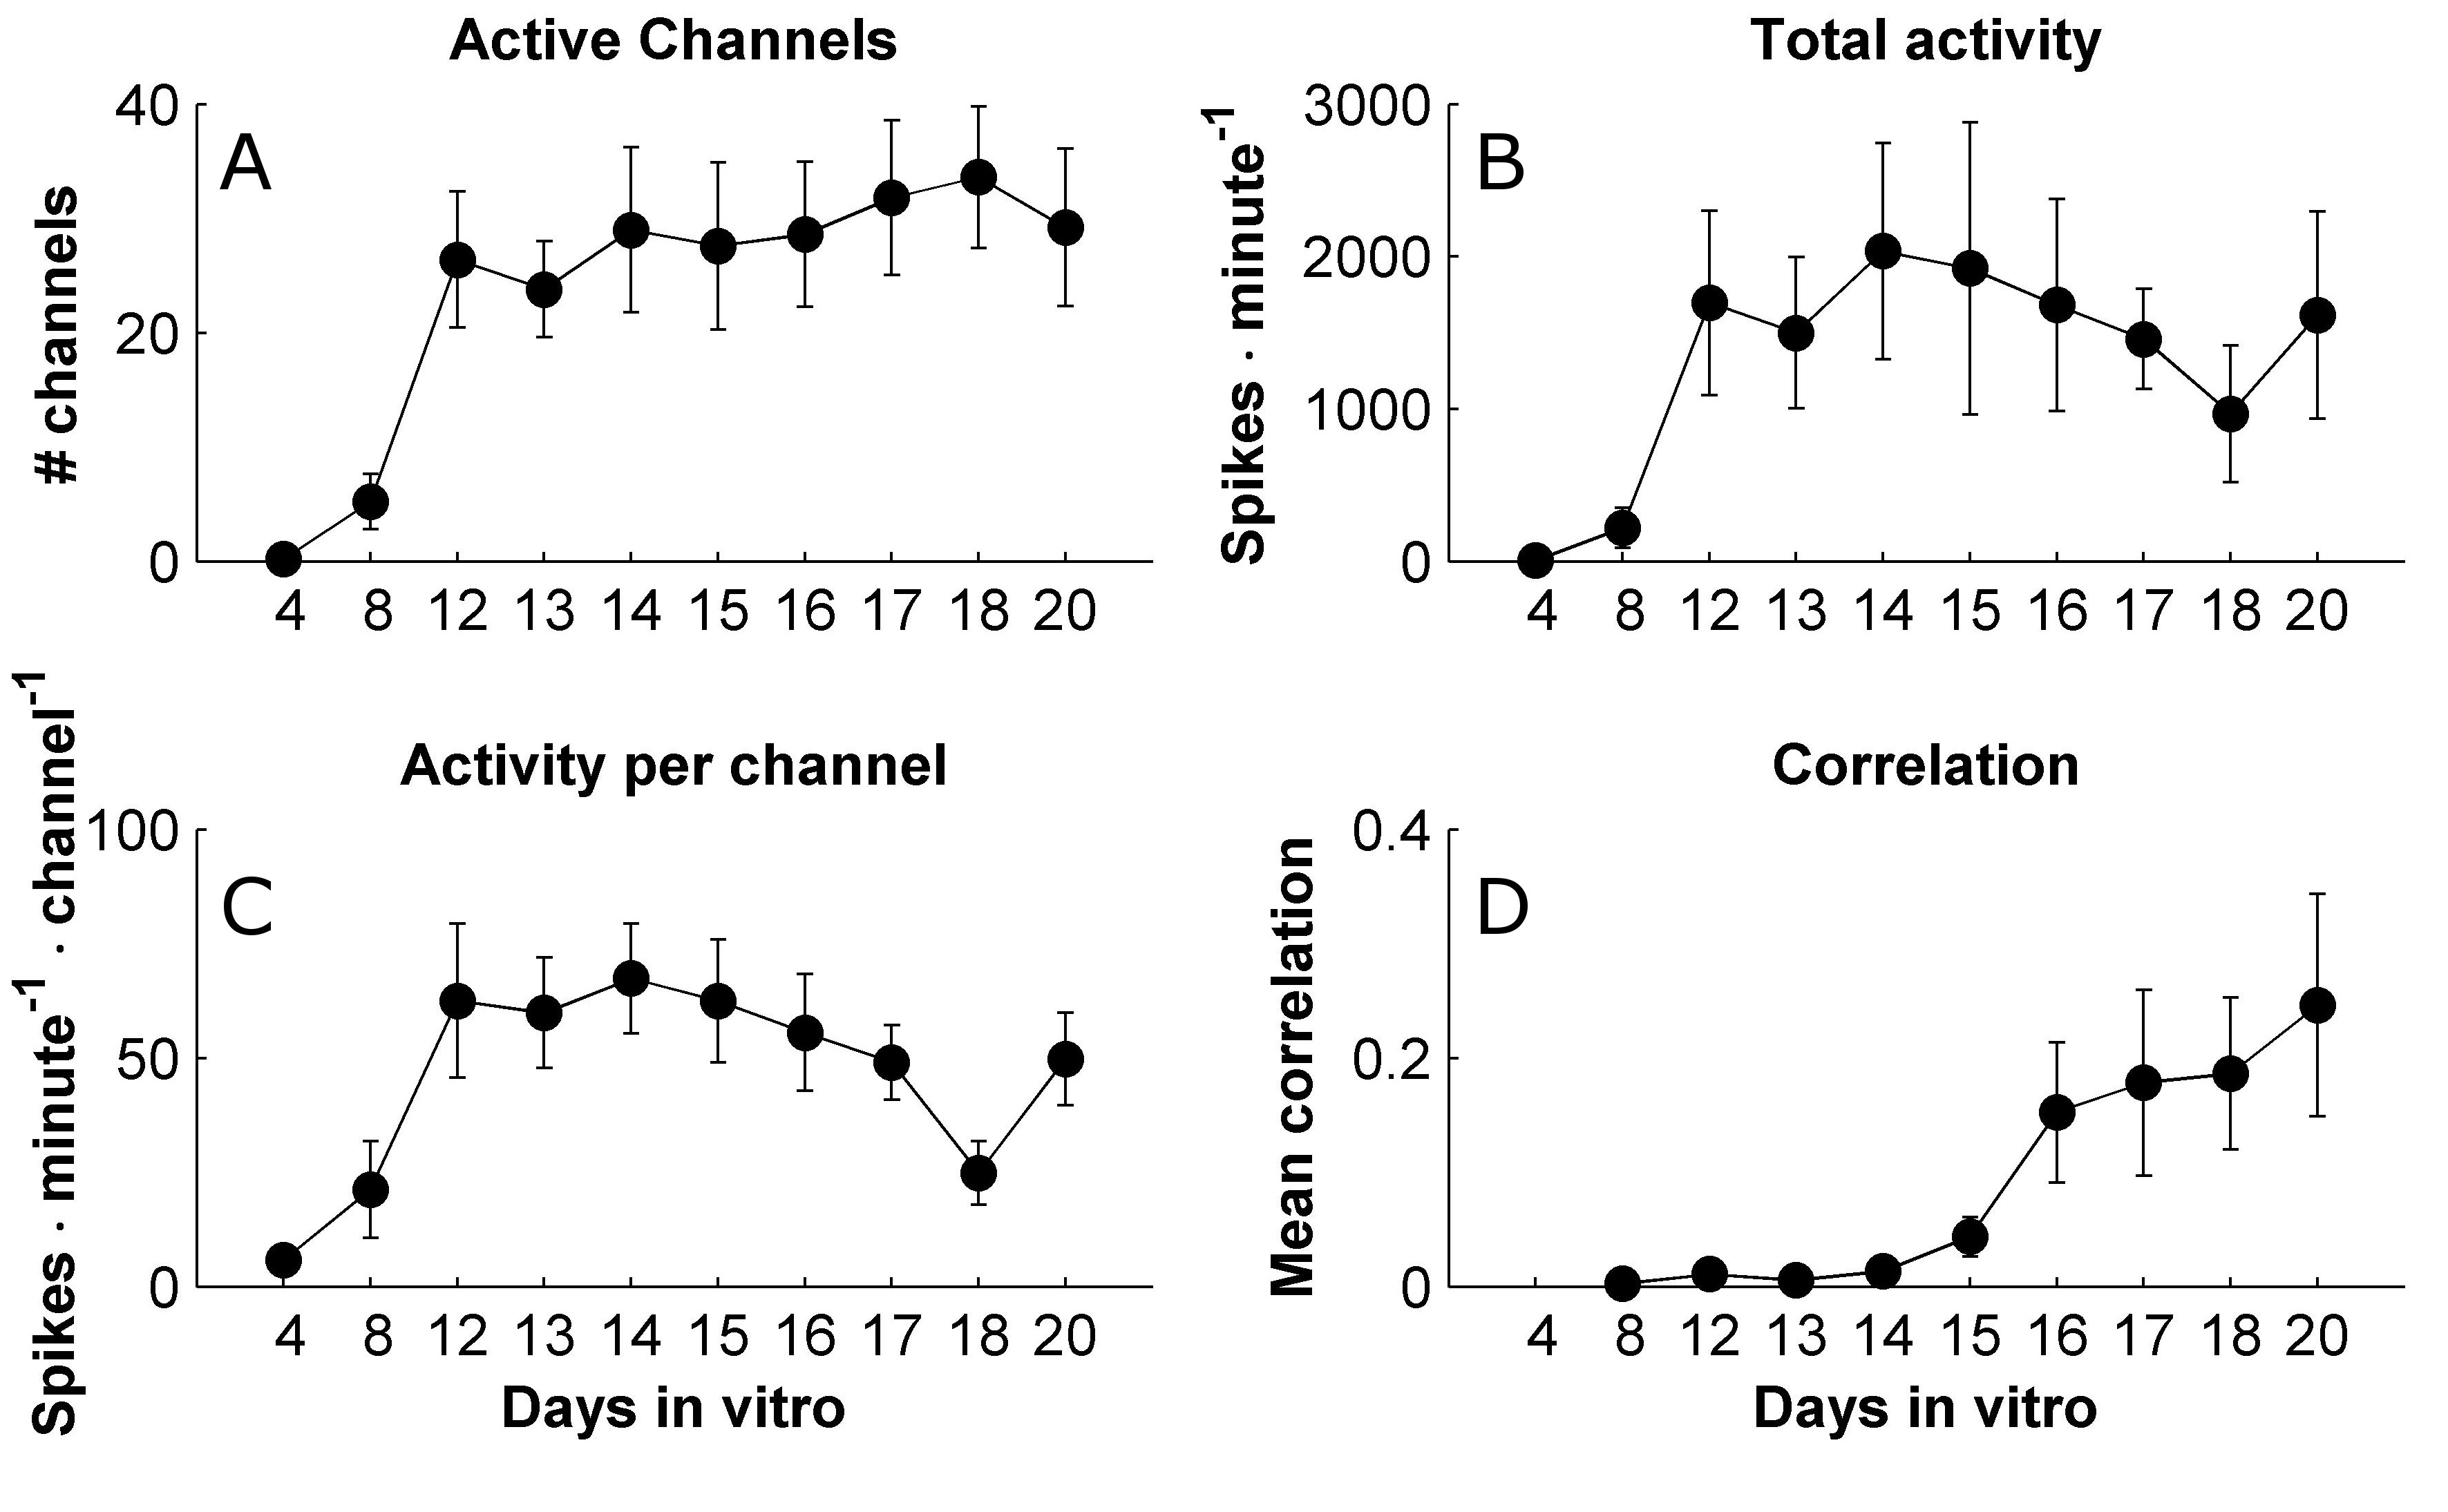
\includegraphics[width=15cm]{chapter3/figures/actMeasures/actMeasures.jpg}

            \caption[Averaged statistics of development of activity measures in mouse cultures]{\textbf{Development of synchronicity in mouse cultures lags after activity.} (A) Development of the number of active channels as a function of culture age. (B) Development of the total number of spikes recorded on all MEA electrodes. (C) Development of the mean neuron firing rate computed as average of firing rate over active channels. (D) Development of mean correlation over time. Mean correlation for a recording is the average of the correlation matrix taken excluding the diagonal. The data are shown as mean and SEM based on n=5 cultures.}
            \label{fig:activity:actMeasures}
        \end{figure}

        The cultures did not become fully active until approximately 2 weeks in culture suggesting that this period of time is required for the seeded progenitor cells to become mature excitable neurons (figure \ref{fig:activity:actMeasures} A-C). This time frame for activity onset is consistent with rat literature \cite{van2004long,wagenaar2006extremely,chiappalone2006dissociated} and is generally accepted with regard to culture electrophysiology where recording are typically performed at least 10 days into development.  After the initial increase, the firing rates (figure \ref{fig:activity:actMeasures} C) stabilize at around \(1 Hz\) and do not exhibit a time dependent trend (1-way ANOVA, p=0.3). The average firing rate per channel is compatible with studies from rat cultures which reported values in the range of \(0.4-1.5 Hz\) \cite{chiappalone2006dissociated,van2004long,corner2002physiological,penn2016network} but the lack of trend is different as rat cultures are reported to show a marked increase in individual firing rates until 21 days and a decline afterwards \cite{chiappalone2006dissociated,bikbaev2015brain}.

        Figure \ref{fig:activity:actMeasures} D shows the development of correlations in our cultures. The correlation value for a given recording is the mean of the correlation matrix (e.g., figure \ref{fig:activity:devExample} C,F and I) without the diagonal. Evidently, despite the stabilization of the mean unit firing rates at day 13 \textit{in vitro}, significant correlations started to arise only from about 17 days \textit{in vitro}. This suggests that the excitability in the cultures is initially controlled by intrinsic homeostatic mechanisms which are later replaced by synaptic drive. Remarkably, the apparent increase in synaptic efficacy is not accompanied by an increase in spiking activity suggesting that the unit mean firing rate of \(1 Hz\) is a controlled quantity which the neurons maintain in the face of a changing network environment around them. Indeed, it has been shown that cultured neurons are capable of rapidly modifying their intrinsic excitability in response to pre-synaptic blockers \cite{penn2016network}.


        To further characterize the spontaneous activity in the cultures we employed a burst detection algorithm as detailed in section \ref{sec:methods:burstDetection} and extracted parameters of burst related measures, shown in figure \ref{fig:activity:burstMeasures}. Not surprisingly, the development of bursting activity followed the same pattern as mean correlation and trailed the development of activity by a few days (figure \ref{fig:activity:burstMeasures} A,D compared to figure \ref{fig:activity:actMeasures} A-C). This separation between measures of individual activity and of of synchronicity underlines the utility of the MEA system in recognizing and disentangling biological processes that are linked. Previous rat cultures studies report that regular bursting is apparent already towards the end of the 2\textsuperscript{nd} week \textit{in vitro} \cite{van2004long,wagenaar2006extremely,chiappalone2006dissociated,bikbaev2015brain} whereas in our mouse data this was rare. In these reports the evolution of bursts appeared to go hand in hand with the evolution of activity, both of which peaked at 21 days \textit{in vitro} and declined afterwards. As bursting behaviour in our data was a few days delayed and started in the middle of the 3\textsuperscript{rd} week \textit{in vitro} it is plausible that a similar trend (but delayed) would be observed had we recorded further into the 4\textsuperscript{th} week.

      \begin{figure}[!htb]
            \centering
            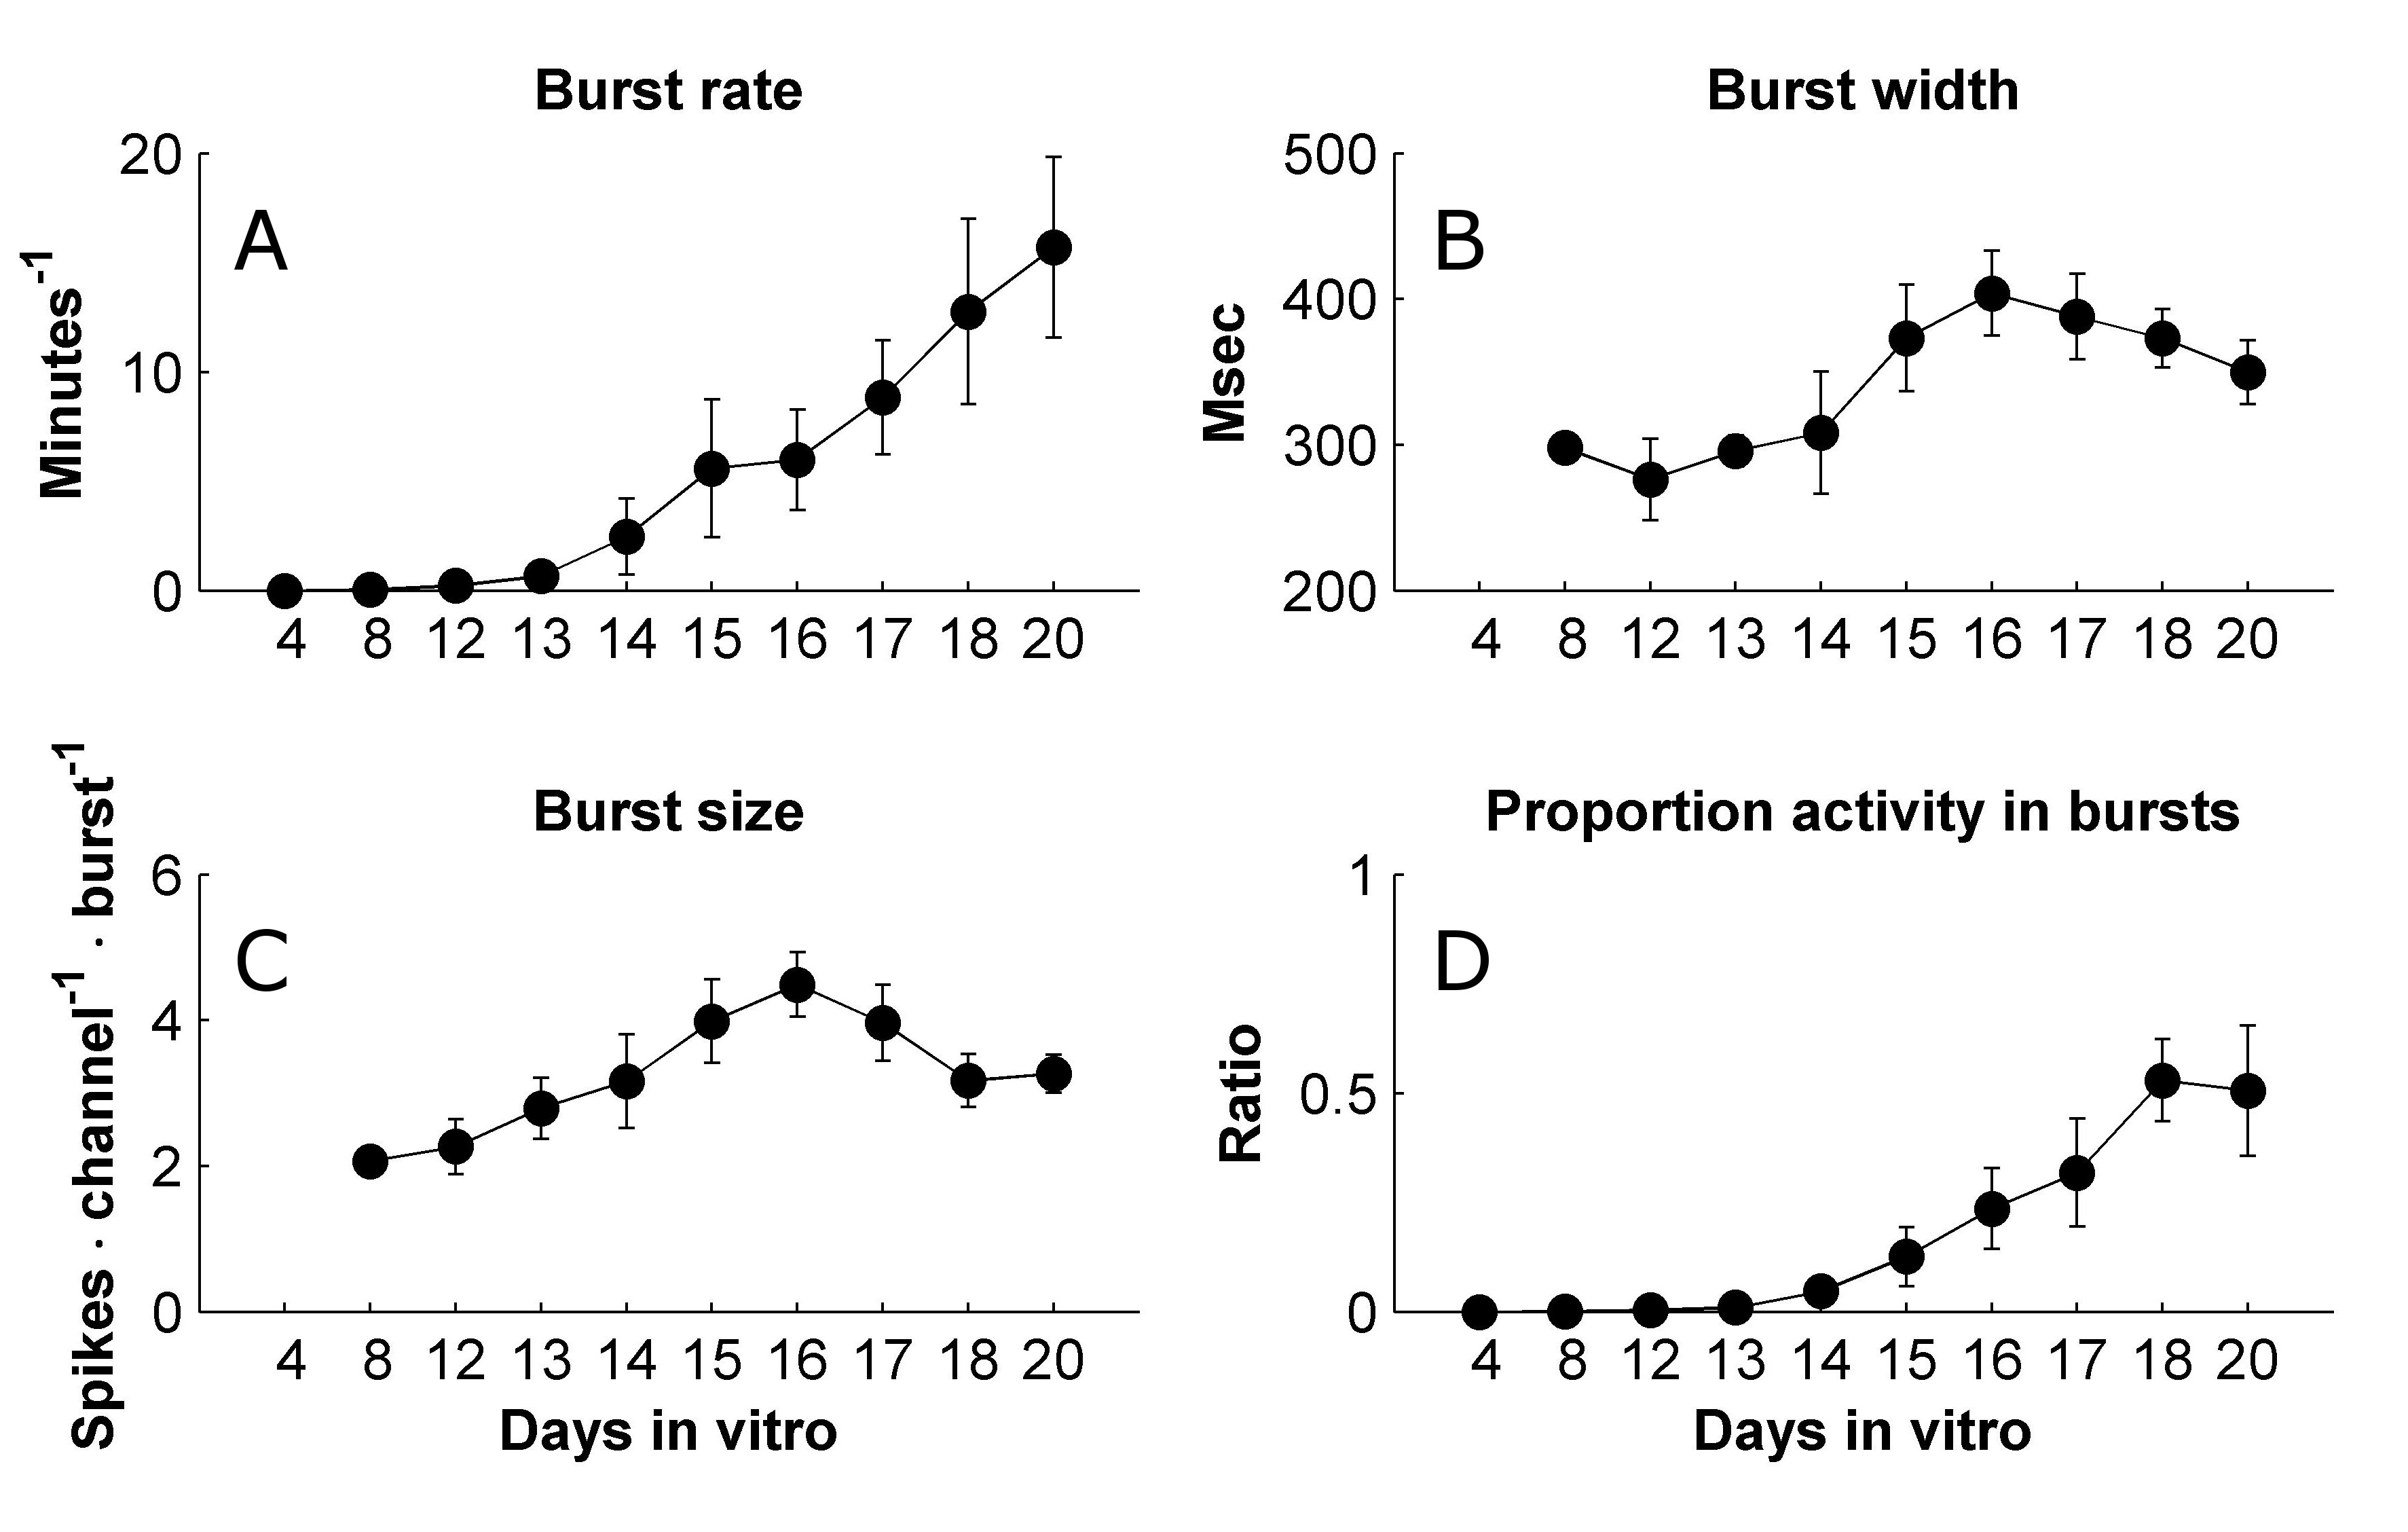
\includegraphics[width=15cm]{chapter3/figures/burstMeasures/burstMeasures.jpg}

            \caption[Averaged statistics of development of bursting measures in mouse cultures]{\textbf{Development of bursting measures in mouse cultures lags behind activity}. (A) Development of burst rate as a function of culture age. (B) Development of burst width. (C) Development of burst size. (D) Development of the ratio between the number of spikes observed within bursting events and the total recorded spikes. Data is shown as mean and SEM based on n=5 cultures.}
            \label{fig:activity:burstMeasures}
        \end{figure}

        It should be noted that the peak burst rate value observed (15 minute\textsuperscript{-1}) was much higher than the one reported for rat cultures at the same age of development (5 minute\textsuperscript{-1}) \cite{chiappalone2006dissociated}. However, we do not believe that this strong discrepancy lies in the difference between the preparations. Rather, our burst detection algorithm (section \ref{sec:methods:burstDetection}) uses an innovative approach for identifying synchronized events. Our method computes surrogate spike rasters with identical firing rates as the original data but without correlations to define the burst detection threshold. The thresholds defined in this way are likely to be tighter than for previous approaches where the thresholds were manually selected based on personal preference of how well they fit the data \cite{wagenaar2006extremely,chiappalone2005burst}. Since our thresholds are based on an objective criteria we argue that the observed burst rate indeed reflects synchronized events and that the rate of these is actually greater than previously reported. In section \ref{sec:activity:mouseRatComp} we will show a direct comparison between mouse and rat data which further supports the above argument.

        Further evidence for delayed synaptic maturation is provided by the burst width and burst size measures. Previous work has established that bursts in naive rat cultures exhibit wide temporal profiles with long tails of spike discharges that could last up to several seconds \cite{chiappalone2006dissociated,van2004longterm}. Over the 3\textsuperscript{rd}-4\textsuperscript{th} weeks the burst profiles become narrow and exhibit increasingly faster termination until saturating in the end of the 4\textsuperscript{th} week. This change is attributed to the development of the GABAergic neurotransmission which was shown to occur 1-2 weeks in delay as compared to the glutamatergic system \cite{ramakers1994activity,swanwick2006development}. Hence it has been postulated that feedback loops operating through inhibitory interneurons become functional only in the aforementioned time period  \cite{van2004long} (3\textsuperscript{rd}-4\textsuperscript{th}, also see an \textit{in vivo} correlate in \cite{hensch2005critical}). In the rat data the bursts show maximal width when they first appear (10-14 days \textit{in vitro}). In our data, a similar trend is observed with peaks appearing in the burst size and burst width measures at 17 days \textit{in vitro}, which is approximately the point when bursting activity became appreciable (time effect was found significant through 1-way ANOVA for both burst size and burst width measures with p=0.035 and 0.028, respectively).

        Another known phenomena where the differences between mouse and rat cultures seem to be manifested are `superbursts'. These refer to periods of elevated activity with epileptiform-like discharges seen in rat cultures in the second and third weeks \textit{in vitro} \cite{wagenaar2006extremely}. These unrestrained firing patterns disappear later on in development, presumably upon the delayed maturation of the inhibitory system mentioned above (see also section \ref{sec:introduction:MEANetwork}). Such superbursts have not been observed in any of the mouse cultures followed here for 3 weeks \textit{in vitro} but were very common in the rat cultures used throughout the following chapters. This observation provides further support to the notion that excitatory synaptic transmission in mouse cultures develops more slowly and might be more effectively balanced by the concurrently developing inhibition.

        Taken together, the results from the spontaneous activity study demonstrate that, on one hand, the development of neurotransmission and synaptic connections in our mouse cultures appears to be delayed between 3 days to one week compared to reported rat cultures. On the other hand, irrespective of the delay, the cultures exhibit all the activity features expected from literature, such as, homeostatic control of excitability, underlying modularity and development of synchronicity and bursting activity which evolve in accordance with the development of the synaptic networks.


    \section{Evoked activity}
    \label{sec:activity:evoked}
    An important feature of the MEA technology is the ability to induce generation of action potentials through injection of a current waveform into the extracellular electrodes. This is an important functionality as it allowed providing input to the network and to influence the culture activity. Past work has provided effective stimulation protocols and showed that short current pulses of several hundred \(\mu s\) can induce individual action potentials as well as a network response \cite{marom2002development,wagenaar2004effective}. This methodology was used to study response properties of single isolated neurons over long periods of time \cite{gal2013entrainment} and how several stimulation pulses interact with each other as a function of temporal proximity \cite{eytan2003selective,weihberger2013quantitative,baljon2009interaction}. This approach was also used to model sensory input by providing more complex spatio-temporal stimulation pattern and examining the extent to which the information present in the input signal can be decoded from the culture activity \cite{marom2009precarious,cozzi2006encoding}. Interestingly, it was shown that high frequency stimulation can break down the synchronized bursting structure of the culture activity, presumably in analogy to brain structures which exhibit higher frequency content and lower synchrony when subjected to a high volume of input during active sensory processing \cite{wagenaar2005controlling}.

        \begin{figure}[!htb]
            \centering
            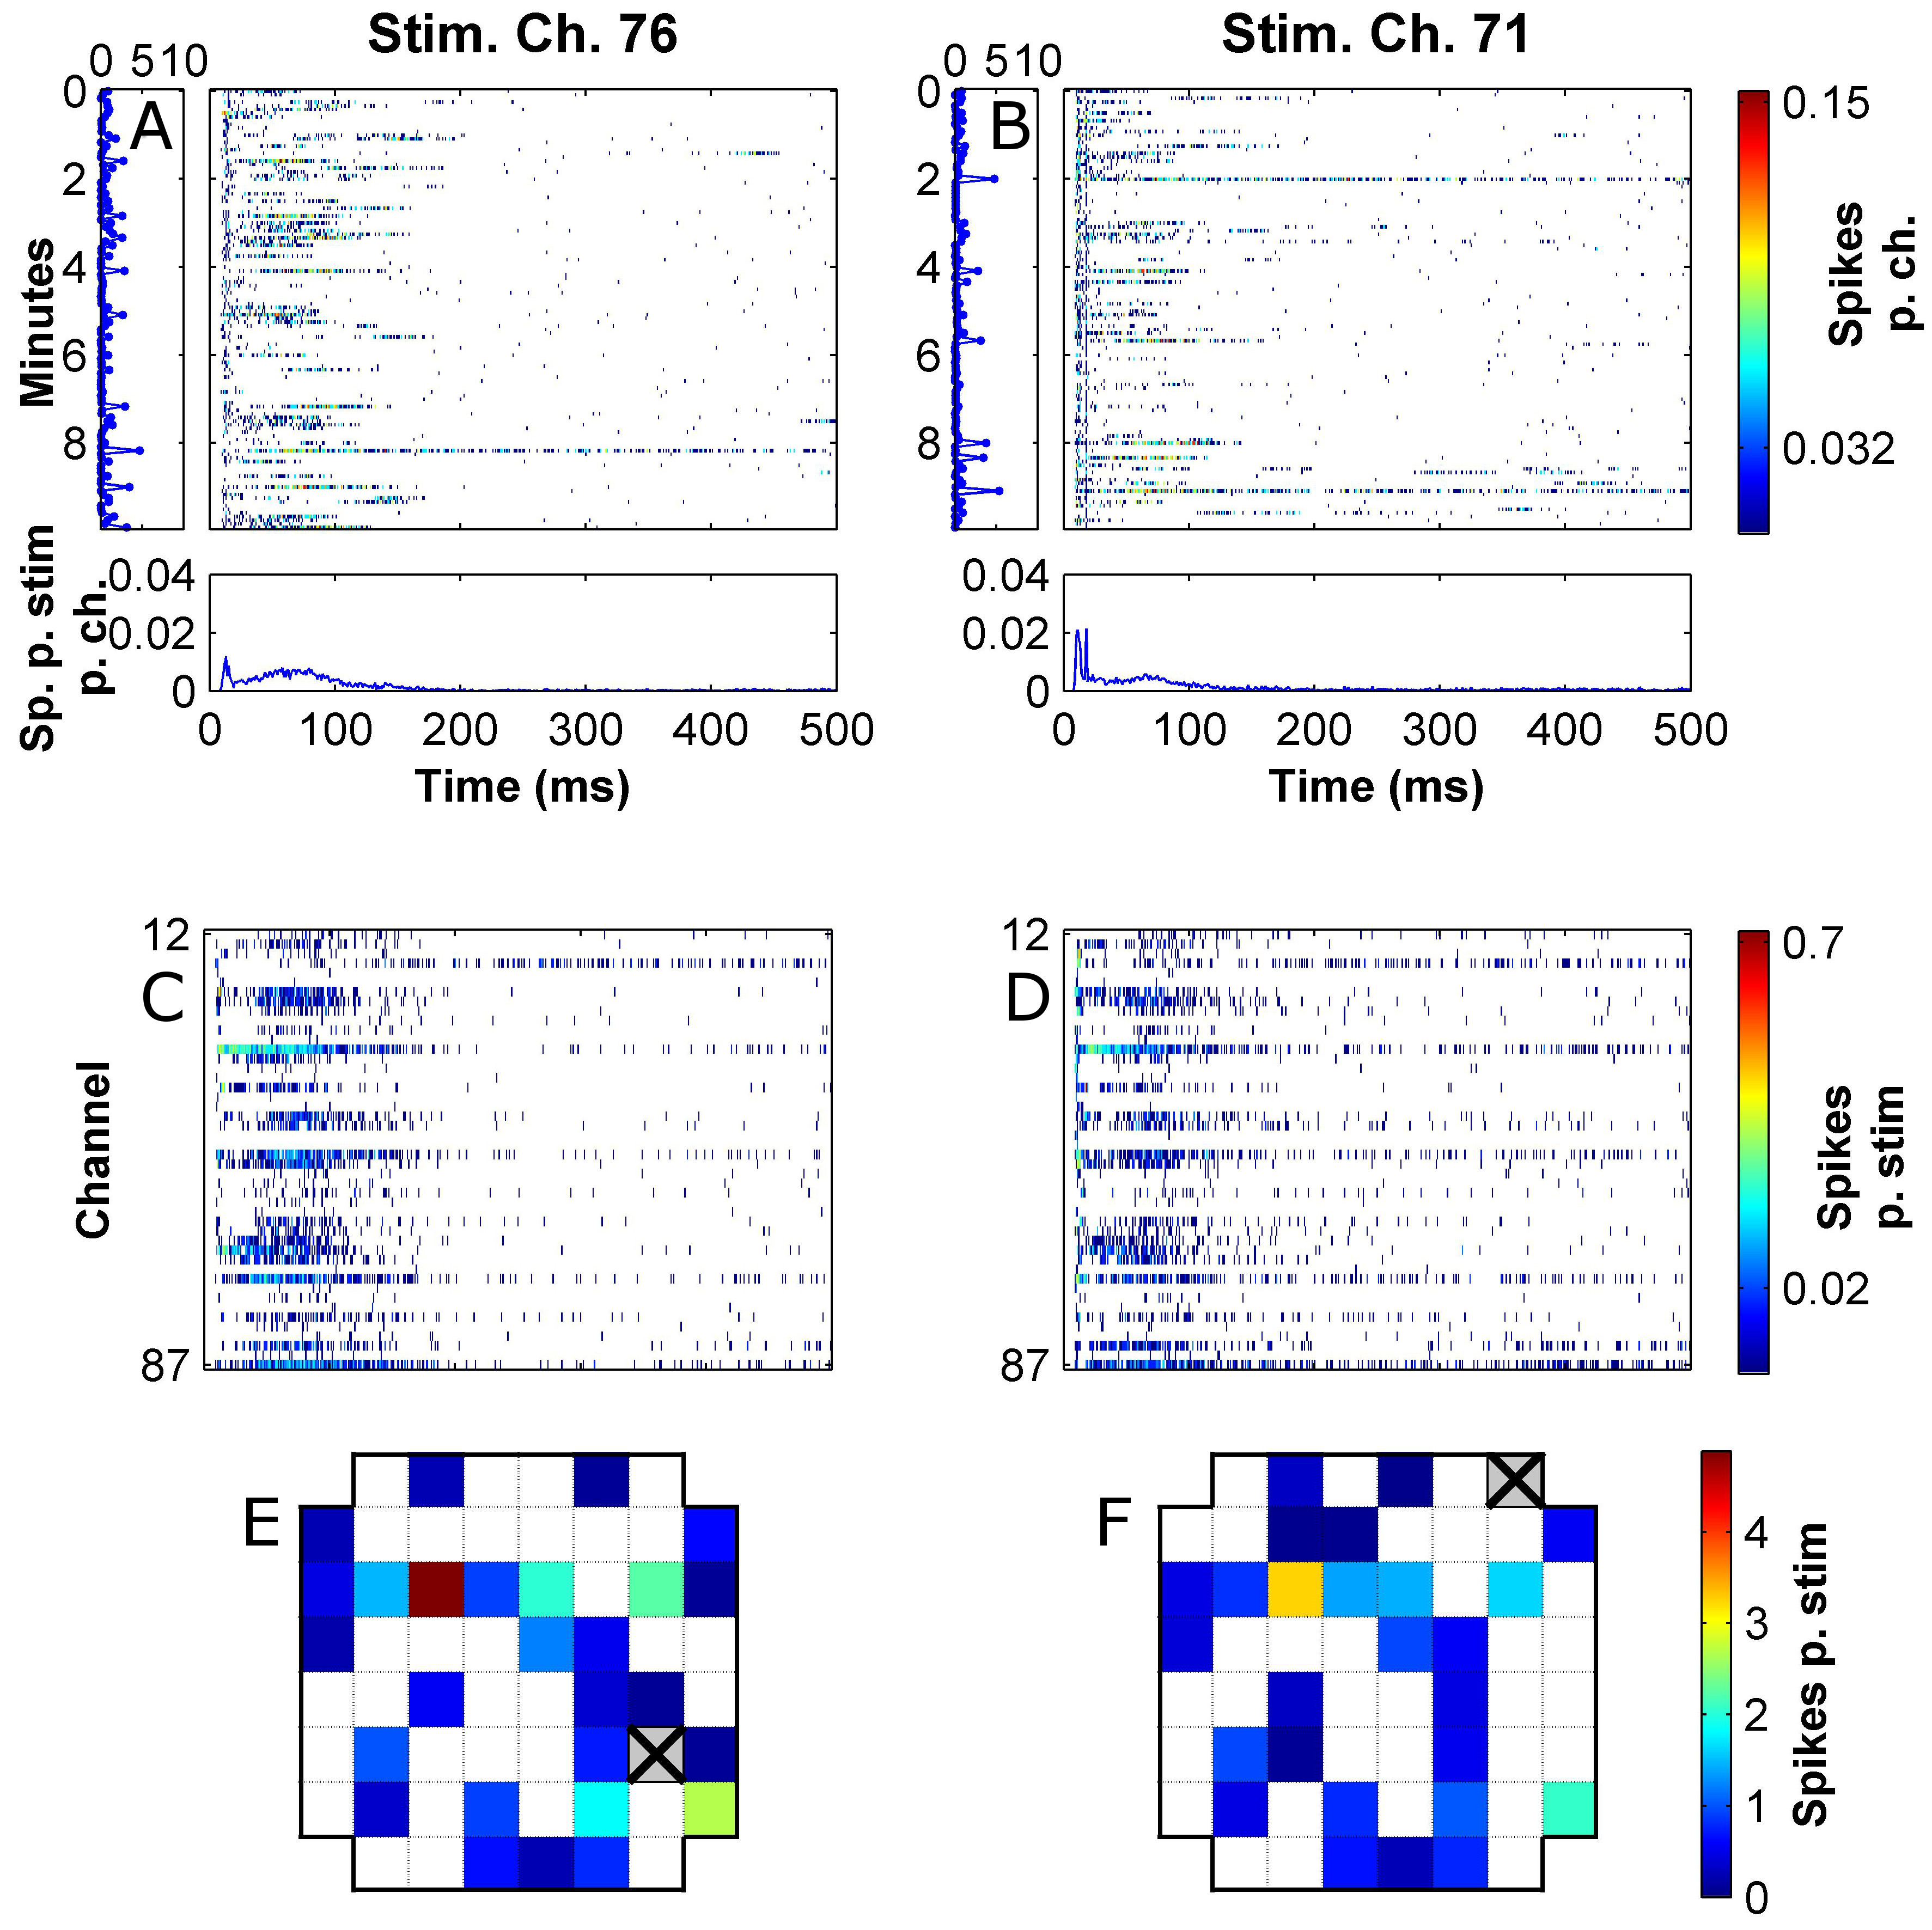
\includegraphics[width=14cm]{chapter3/figures/stimExample/stimExample.jpg}

            \caption[Example of responses to test stimuli applied at 2 different electrodes]{\textbf{Stimulation pulses at different electrodes vary in direct responses but produce a similar reverberative responses.} Test stimuli were applied every 5 seconds. (A-B) Main panel: Each line is a response raster for one test stimulus averaged over all channels. Left panel shows the sums of the responses shown in the main panel over the post stimulus observation time window (i.e., number of spikes per channel observed in 500 ms period post stimulation). Bottom panel shows the average of the response rasters over all stimuli. This is the PSTH. (C-D) Spatially resolved PSTHs, i.e., each line is a channel PSTH. The spatial profiles of the responses to the different stimulation sites are visually similar. (E-F) Stimulation response maps showing the sums of the PSTHs in (C-D) in the actual spatial locations. These response maps only show channels with a stimulation response that is significantly higher than background spontaneous activity for that channel (see section \ref{sec:methods:stim} for selection procedure). Stimulating electrodes are marked by an X on a gray background. A,C,E and B,D,F show response data for two stimulation sessions applied to two different electrodes (indicated in E,F) run one after the other in succession on the same culture. All raster plots use 1 \(1ms\) bins.}
            \label{fig:activity:stimExample}
        \end{figure}

    To demonstrate that our system is able to effectively interface with the culture and provide input, we present data from a stimulation session where 120 test pulses were applied every 5 seconds to a single electrode (see section \ref{sec:methods:stim} for technical details). Data for two distinct stimulation sites (electrodes) are shown. Figure \ref{fig:activity:stimExample} A-B shows raster plots of the stimulation responses (at the different sites) averaged over all channels in a \(500 ms\) window after the stimulation pulse, as well as a PSTH, which is essentially the average of all individual responses (post stimulus time histogram). The PSTH was typical to what is normally observed in these preparations: a bimodal curve with a sharp peak observed within the first \(25 ms\) after stimulation and a second, significantly wider and less defined peak which typically lasts about \(200 ms\) after stimulation. The first peak is considered to represent direct responses, i.e., spikes elicited directly as a result of the stimulation pulse without synaptic mediation. The second peak is thought to be a manifestation of a multi-synaptic reverberating activity in response to the first step of activation. Indeed, it is evident from the response rasters that the first stage of response is significantly more repeatable than the second one which was not always present. This is compatible with the above interpretation as direct responses are spikes generated due to a stimulation induced localized depolarization and depend only the specific biophysics and geometry of the neuron so they are expected to occur at a set delay and with low jitter. The reverberating response, on the other hand, is a complex phenomena which depends on the network state preceding the stimulus so it stands to reason that it would show large variability or even fail to propagate on occasion. Nevertheless, it should be noted that even the direct responses were far from operating at a 100\% success rate, a single neuron reproducibility issue that has been under much debate within the neuroscience community \cite{mainen1995reliability,gal2013entrainment}.

    Comparing between the responses to the two stimulation sites it is evident that they differed in direct responses with stimulations in channel 71 producing a second direct response peak which is also observable as a vertical line in the response rasters. The reverberating response did not show conspicuous differences in shape or latency although it seemed somewhat smaller. Another view on the differences between the two stimulation sites is given in figure \ref{fig:activity:stimExample} C-F which show spatially resolved response rasters (i.e., PSTHs of individiual channels) and response maps for all participating channels, averaged over the stimulations. The spatial response profile appears to be very similar when comparing the two different stimulation electrodes - each channel showed a similar strength and duration of activation. There are some differences in latency but these were relatively unpronounced, at least to the naked eye. Although we did not study this in depth, it was our impression that different stimulation electrodes differ in mainly whether they are were at all able to produce a reverberating response. However, once this response was elicited it seems to be stereotypical, i.e., each culture develops to take on an particular identity which is elicited whenever a synchronized burst occurs regardless of the site of induction or if it is spontaneous or evoked. It has been suggested that the lack of sensory input during culture development drives it into a degenerate state of over connectedness which might explain this rigidity. On the other hand, it should be noted that distinct yet overlapping responses to different stimulation sites have been reported \cite{wagenaar2006searching}. Additionally, decoding of spatial stimulation information from culture data has been successfully demonstrated \cite{kermany2010tradeoffs} so this system might nevertheless model genuine neural coding mechanisms from \textit{in vivo}.

    \section{Plasticity induction in the presence of dopamine}
    Mature neuronal cultures abide to the principles of spike timing dependent plasticity (STDP), demonstrated in a paired pulse paradigm \cite{bi1998synaptic}. This observation has raised the interesting possibility that neuronal cultures grown on multi electrode arrays could be used to study how plasticity operates at the network level. This sparked a substantial body of work to devise paradigms for induction and observation of plasticity using just extracellular network recordings and stimulations. Initial efforts have focused on brief tetanic stimulations inspired by the original experiments discovering LTP and which used this stimulation protocol \cite{bliss1973long}. Positive reports employing tetanus based induction have reported either a generalized potentiation in evoked responses which could be observed using simple measures such as summated response over all MEA electrodes \cite{chiappalone2008network,hamilton2015time,ruaro2005toward} or more subtle effect that did not involve global change but rather antagonistic changes to the different channels and required more sophisticated multi-variate analyses to observe \cite{jimbo1999simultaneous,le2015repeated,madhavan2007plasticity}. The latter type of plasticity was observed both in evoked responses as well as in spontaneous activity. Indeed that tetanus induces a global potentiation is not surprising given that the original LTP experiments involved potentiation in the LFP measurements which represent large populations of neurons. However, it is known that neuronal systems employ homeostatic mechanisms to keep the general excitation levels constant \cite{turrigiano1999homeostatic} so such extreme modifications to activity are likely to be unphysiological. In that sense it is interesting that more subtle forms of plasticity are observed in the multi dimensional aspect of the activity. However, it is unclear why similar protocols produce such differences in outcome in different studies and different labs. Later work has shown that low frequency stimulation protocols can also induce changes in spontaneous activity of the subtle type \cite{le2015repeated,vajda2008low}. This result is interesting as natural input during real-life behavioural learning is probably more similar to such low frequency signals than to tetanus. Obviously, behaviour in general and learning in particular are a closed loop process and this was modeled, to a certain extent, with feedback systems where the stimulation pattern was directly informed by the preceding neuronal activity \cite{bakkum2008spatio,shahaf2001learning}. These important works showed that the direction and extent of plasticity can be controlled to follow bespoke criteria and therefore established that they are indeed relevant for goal directed learning.

    As mentioned above, the quest to find plasticity in neuronal cultures grown in MEAs has produced successes but also contradictory, controversial and negative reports \cite{wagenaar2006searching,le2009slow}. Here we provide our own contribution to the discussion by applying one of the reported protocols
    to our mouse cultures and checking for plasticity. Additionally, as reviewed in section \ref{sec:introduction:neuromodulators}, neuromodulators have been shown to be strongly associated with neuronal plasticity and their presence or absence can strongly affect the direction of change (i.e., potentiation or depression) or even abolish it altogether (reviewed in section \ref{sec:introduction:neuromodulators}. Consequently it has been suggested that dopamine signalling is a missing ingredient required to facilitate consistent plastic processes in culture. Further support for this notion was provided by a culture study showing that dopamine modulates of the effective STDP window using intracellular recordings \cite{zhang2009gain}. Since neuromodulators have not been used in conjunction with plasticity and neuronal cultures on MEAs we decided to include a phase within our protocol where dopamine is introduced just for the induction period and washed away afterwards. The reason for washing the dopamine away was to avoid mistaking its direct modulation of the activity to be synaptic plasticity. Additionally, since neuromodulators signal the occurrence of a salient or rewarding events we intended this paradigm to model a situation where such rewarding event occurs during the tetanus.

    We elected to use a tetanus induction protocol based on \cite{chiappalone2008network}. The reasons for selecting this protocol are as follows: Firstly, some of the past plasticity work on MEAs did not include a control to verify that the observed changes are due to the stimulated activity and not an artefact. Although this may seem unscientific it is a consequence of the nature of the system where each sample takes a long time to produce, maintain and measure. As a result, achieving a high n-number for both experiment and control is in some cases impractical. Our protocol works around this by exploiting the fact that neuronal cultures on MEAs can be used continuously for many recordings without compromise so we ran all experimental and control sessions on the same culture consecutively. Secondly, more complicated protocols such as the ones that apply stimulation in feedback from the recorded activity would require a sophisticated drug application system which is not currently available. This protocol includes a tetanus epoch of just a few minutes which offers a convenient time frame for manual addition and washing away of the drug.

        \label{sec:activity:plasticityProtocol}
        \begin{figure}[!htb]
            \centering
            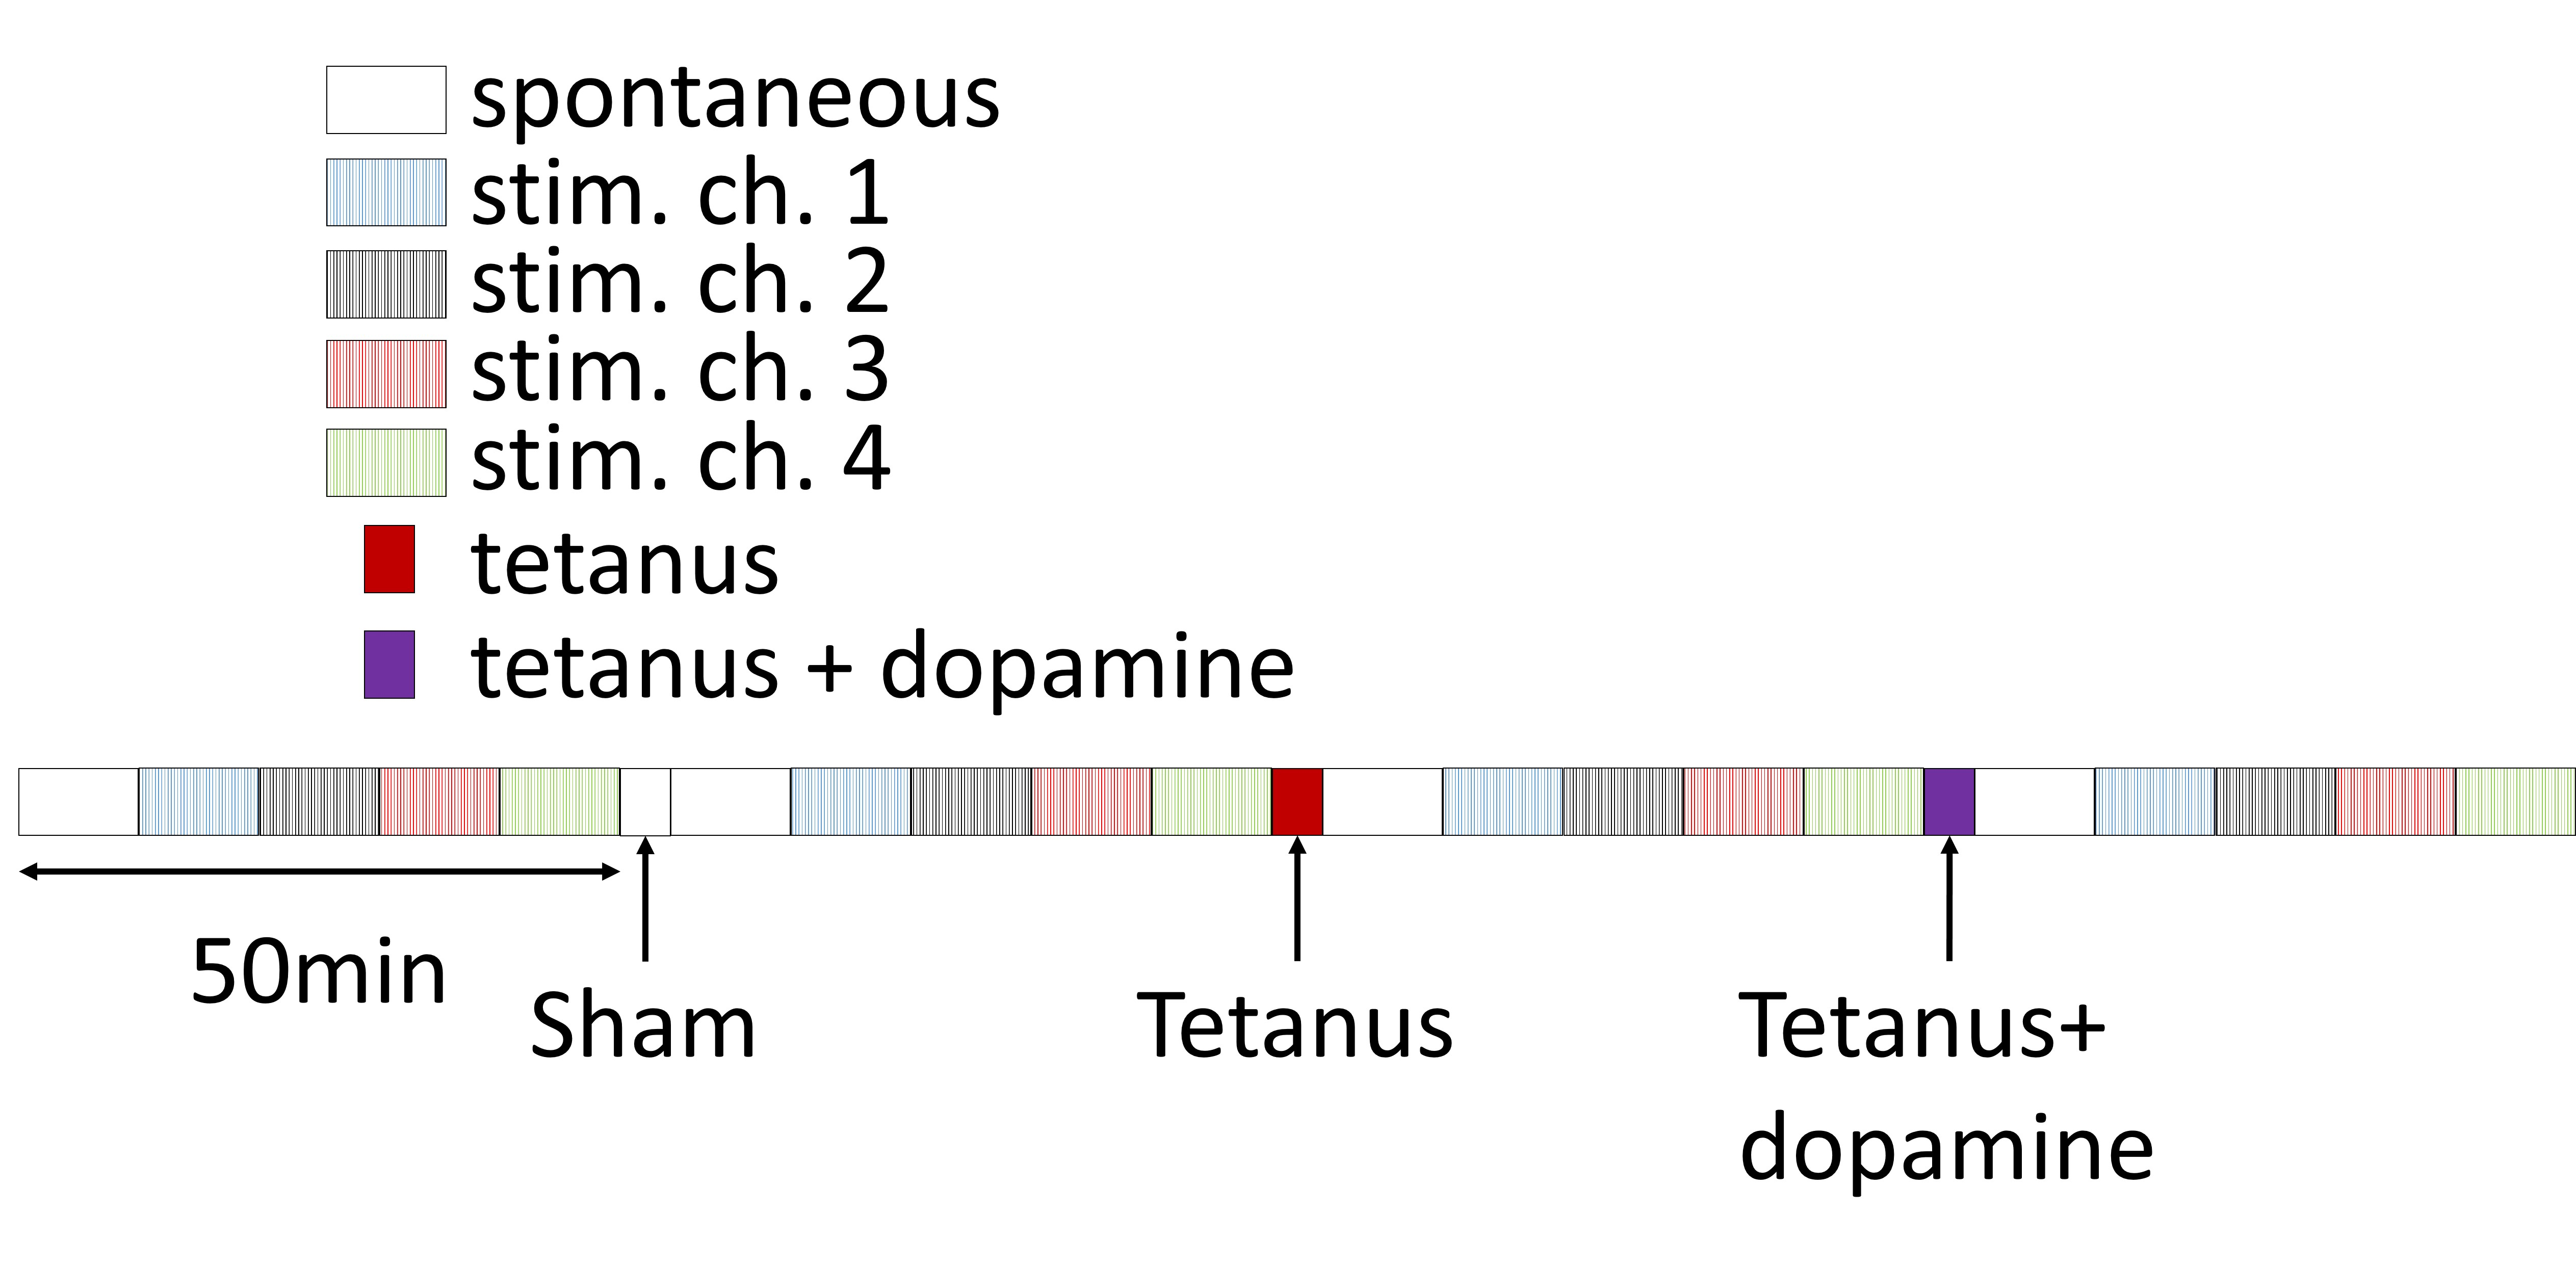
\includegraphics[width=15cm]{chapter3/figures/ExpOutline/expOutlineTet.jpg}

            \caption[Outline of the combined dopamine-and-tetanus-induced open bath plasticity experiments]{\textbf{Outline of the combined dopamine and tetanus open bath plasticity experiments.}}
            \label{fig:activity:expOutline}
        \end{figure}

    Figure \ref{fig:activity:expOutline} shows a schematic of the experiment. The protocol catered for examination of both spontaneous activity and evoked responses. Each measurement epoch comprised a period of 10 minute recording spontaneous activity, followed by 4 x 10 minute periods of recording under 0.2 Hz test stimuli applied at 4 different electrodes, respectively. The electrode identities and amplitudes of test stimuli were selected to produce obvious evoked responses based on a pre-experiment examination. The measurement epochs were separated by 3 induction epoch running an 'associative tetanus' as proposed by \cite{chiappalone2008network}. 'Associative tetanus' is a stimulation paradigm designed to induce an association between two stimulated populations. The primary channel produces a tetanus pulse train consisting 50 pulse sets at \(0.2 Hz\) each consisting of 50 pulses at \(20 Hz\). The secondary channel produces 50 single pulses at 0.2 Hz in phase with the tetanus pulse sets, i.e., each stimulation pulse in the secondary channel is timed to occur in the middle of a set in the primary channel. The primary and secondary channels were selected randomly out of the 4 stimulation channels used in the measurement epochs. The 3 induction epochs are as follows: (1) a sham (control) 'associative tetanus' executed by the signal generator with pulses of \(0 mV\) amplitude. (2) An actual 'associative tetanus' where the amplitudes for the primary and secondary channels are the same as those used in the test stimuli in the same channels during the measurement epochs. (3) An 'associative tetanus' as above where half of the culture media (\(0.5 ml\)) was first removed for later use and \(100 \mu M\) dopamine was added. After the termination of the tetanus the dopamine containing media was replaced with the portion earlier removed and the final examination epoch was carried through. It should be noted that removal of half of the media during the 3\textsuperscript{rd} induction epoch caused a slight but noticeable increase in the recording noise so the spike detection thresholds in the earlier measurement epochs were matched to the last one to avoid biasing of the results.

    \subsection{Examining changes in response to stimulation}
    Figure \ref{fig:activity:tetStimChange} shows example stimulation response data for the 4 measurement epochs in one of the tested cultures. Data is presented as explained in section \ref{sec:activity:evoked}. Baseline refers to the initial measurement epoch performed prior to any induction epoch. Control refers to the epoch taking place after the sham tetanus and the differences from the preceding epoch reflect spontaneous deviations in the culture activity. Tetanus and tetanus + dopamine are the epochs following the genuine induction phases. The differences between these experimental epochs and their immediate predecessors are compared to the difference between the control and baseline epochs so as to capture the effect of the induction. The baseline, control and tetanus epochs all show a similar PSTH profile and similar channel rasters. However, there are also some noticeable differences. For example, the latency of the reverberating response seems to increase approximately half way through the control epoch, a change that is carried over to the tetanus epoch. Additionally, the reverberating phase in the control PSTH is smaller than in the baseline and this is observed as reduced intensity in some of the channel rasters. These spontaneously occurring changes (i.e., not associated with the tetanus induction) highlight the importance of employing such control epochs to assess how activity features change spontaneously.

        \begin{figure}[!htb]
            \centering
            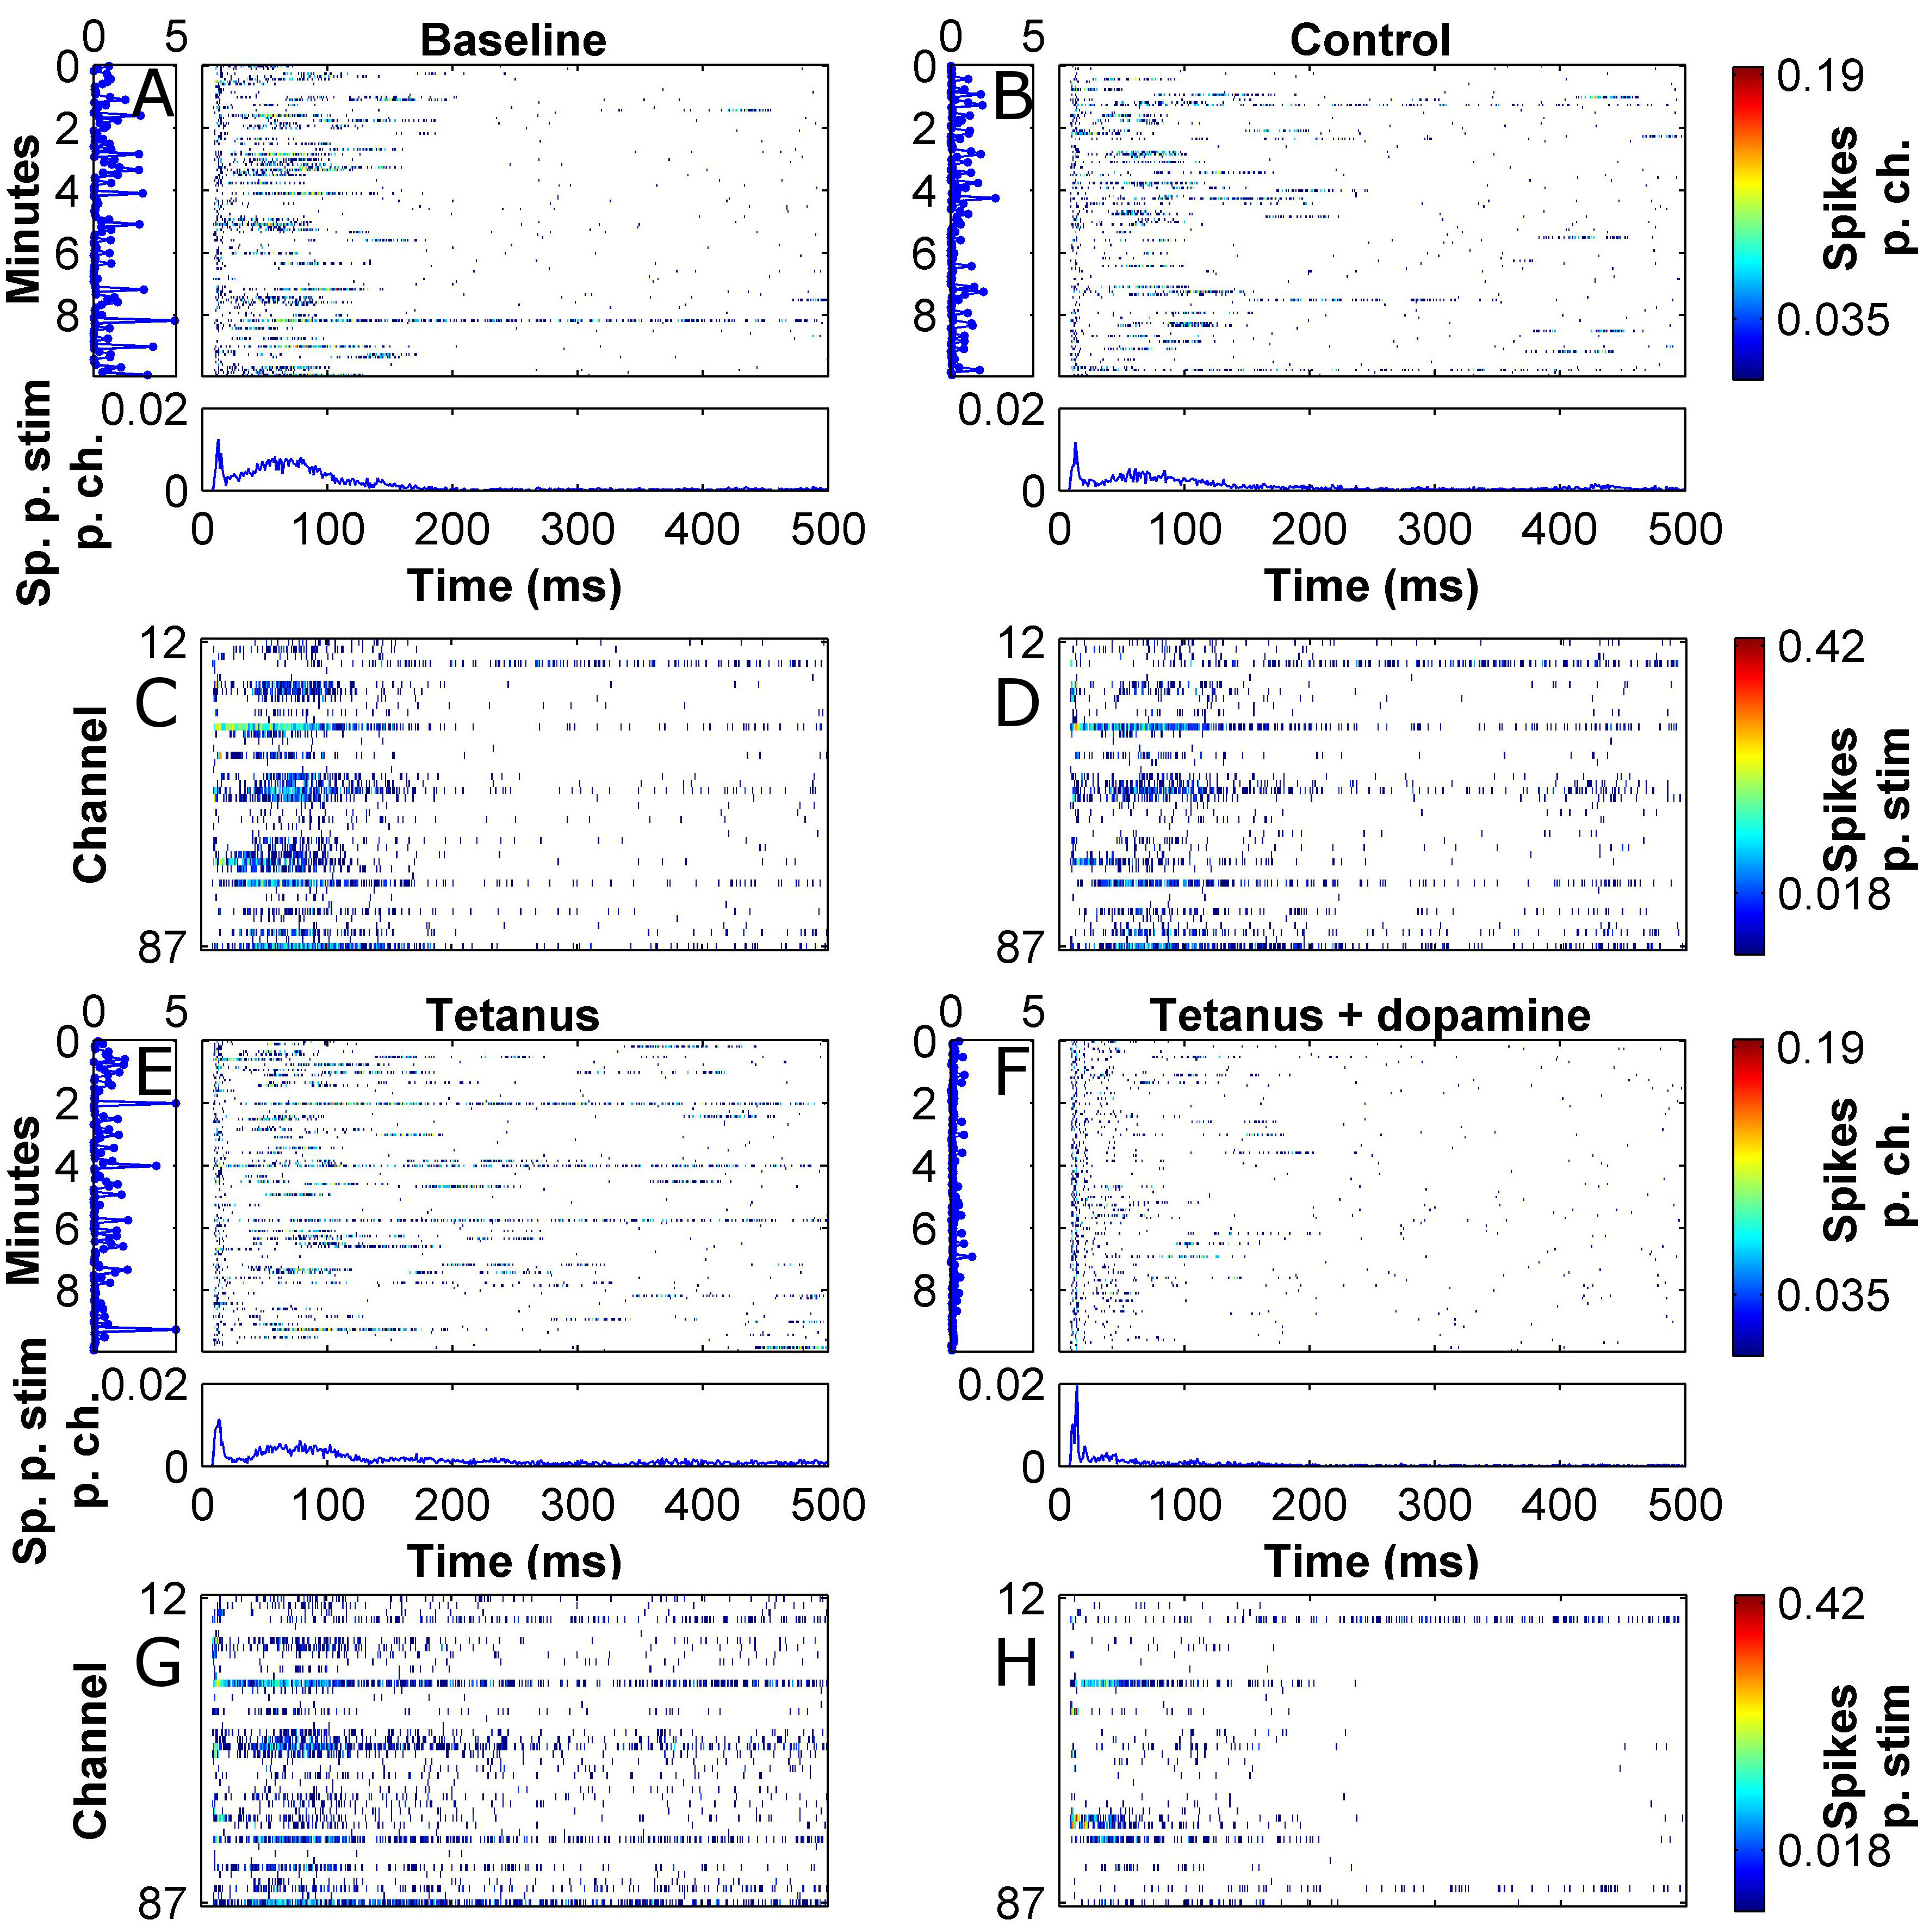
\includegraphics[width=15cm]{chapter3/figures/tetStimChange/tetStimChange.jpg}

            \caption[Example response rasters from the combined dopamine and tetanus plasticity induction experiment]{\textbf{Tetanus combined with a dopamine pulse but not tetanus alone induces a depression of evoked responses.} (A,B,E,F) Response rasters from the first stimulating electrode of each of the measurement epochs of the induction experiment. These are stimulation resolved (i.e., each line is a response to a single stimulation averaged over all the recording channels). (C,D,G,H) Channel-resolved response rasters of the same stimulation epochs. See caption of figure \ref{fig:activity:stimExample} for further details. Note an obvious decrease of evoked responses intensity following the tetanus induction in the presence of dopamine.}
            \label{fig:activity:tetStimChange}
        \end{figure}

    The tetanus + dopamine induction resulted in significantly more pronounced modifications to the evoked responses than the preceding inductions. The most obvious difference was the global reduction to the reverberating response in the PSTH. Most of the channels showed a marked decrease in intensity of responses although there were a few that actually increased. Another notable difference is that the direct response had become sharper. This global decrease in response is evident in the response maps in figure \ref{fig:activity:tetMapChange} where the number of responsive channels and their firing rate is markedly smaller after the tetanus + dopamine induction (recall that the response maps show only channels with significantly higher stimulation associated response in comparison with spontaneous activity).

        \begin{figure}[!htb]
            \centering
            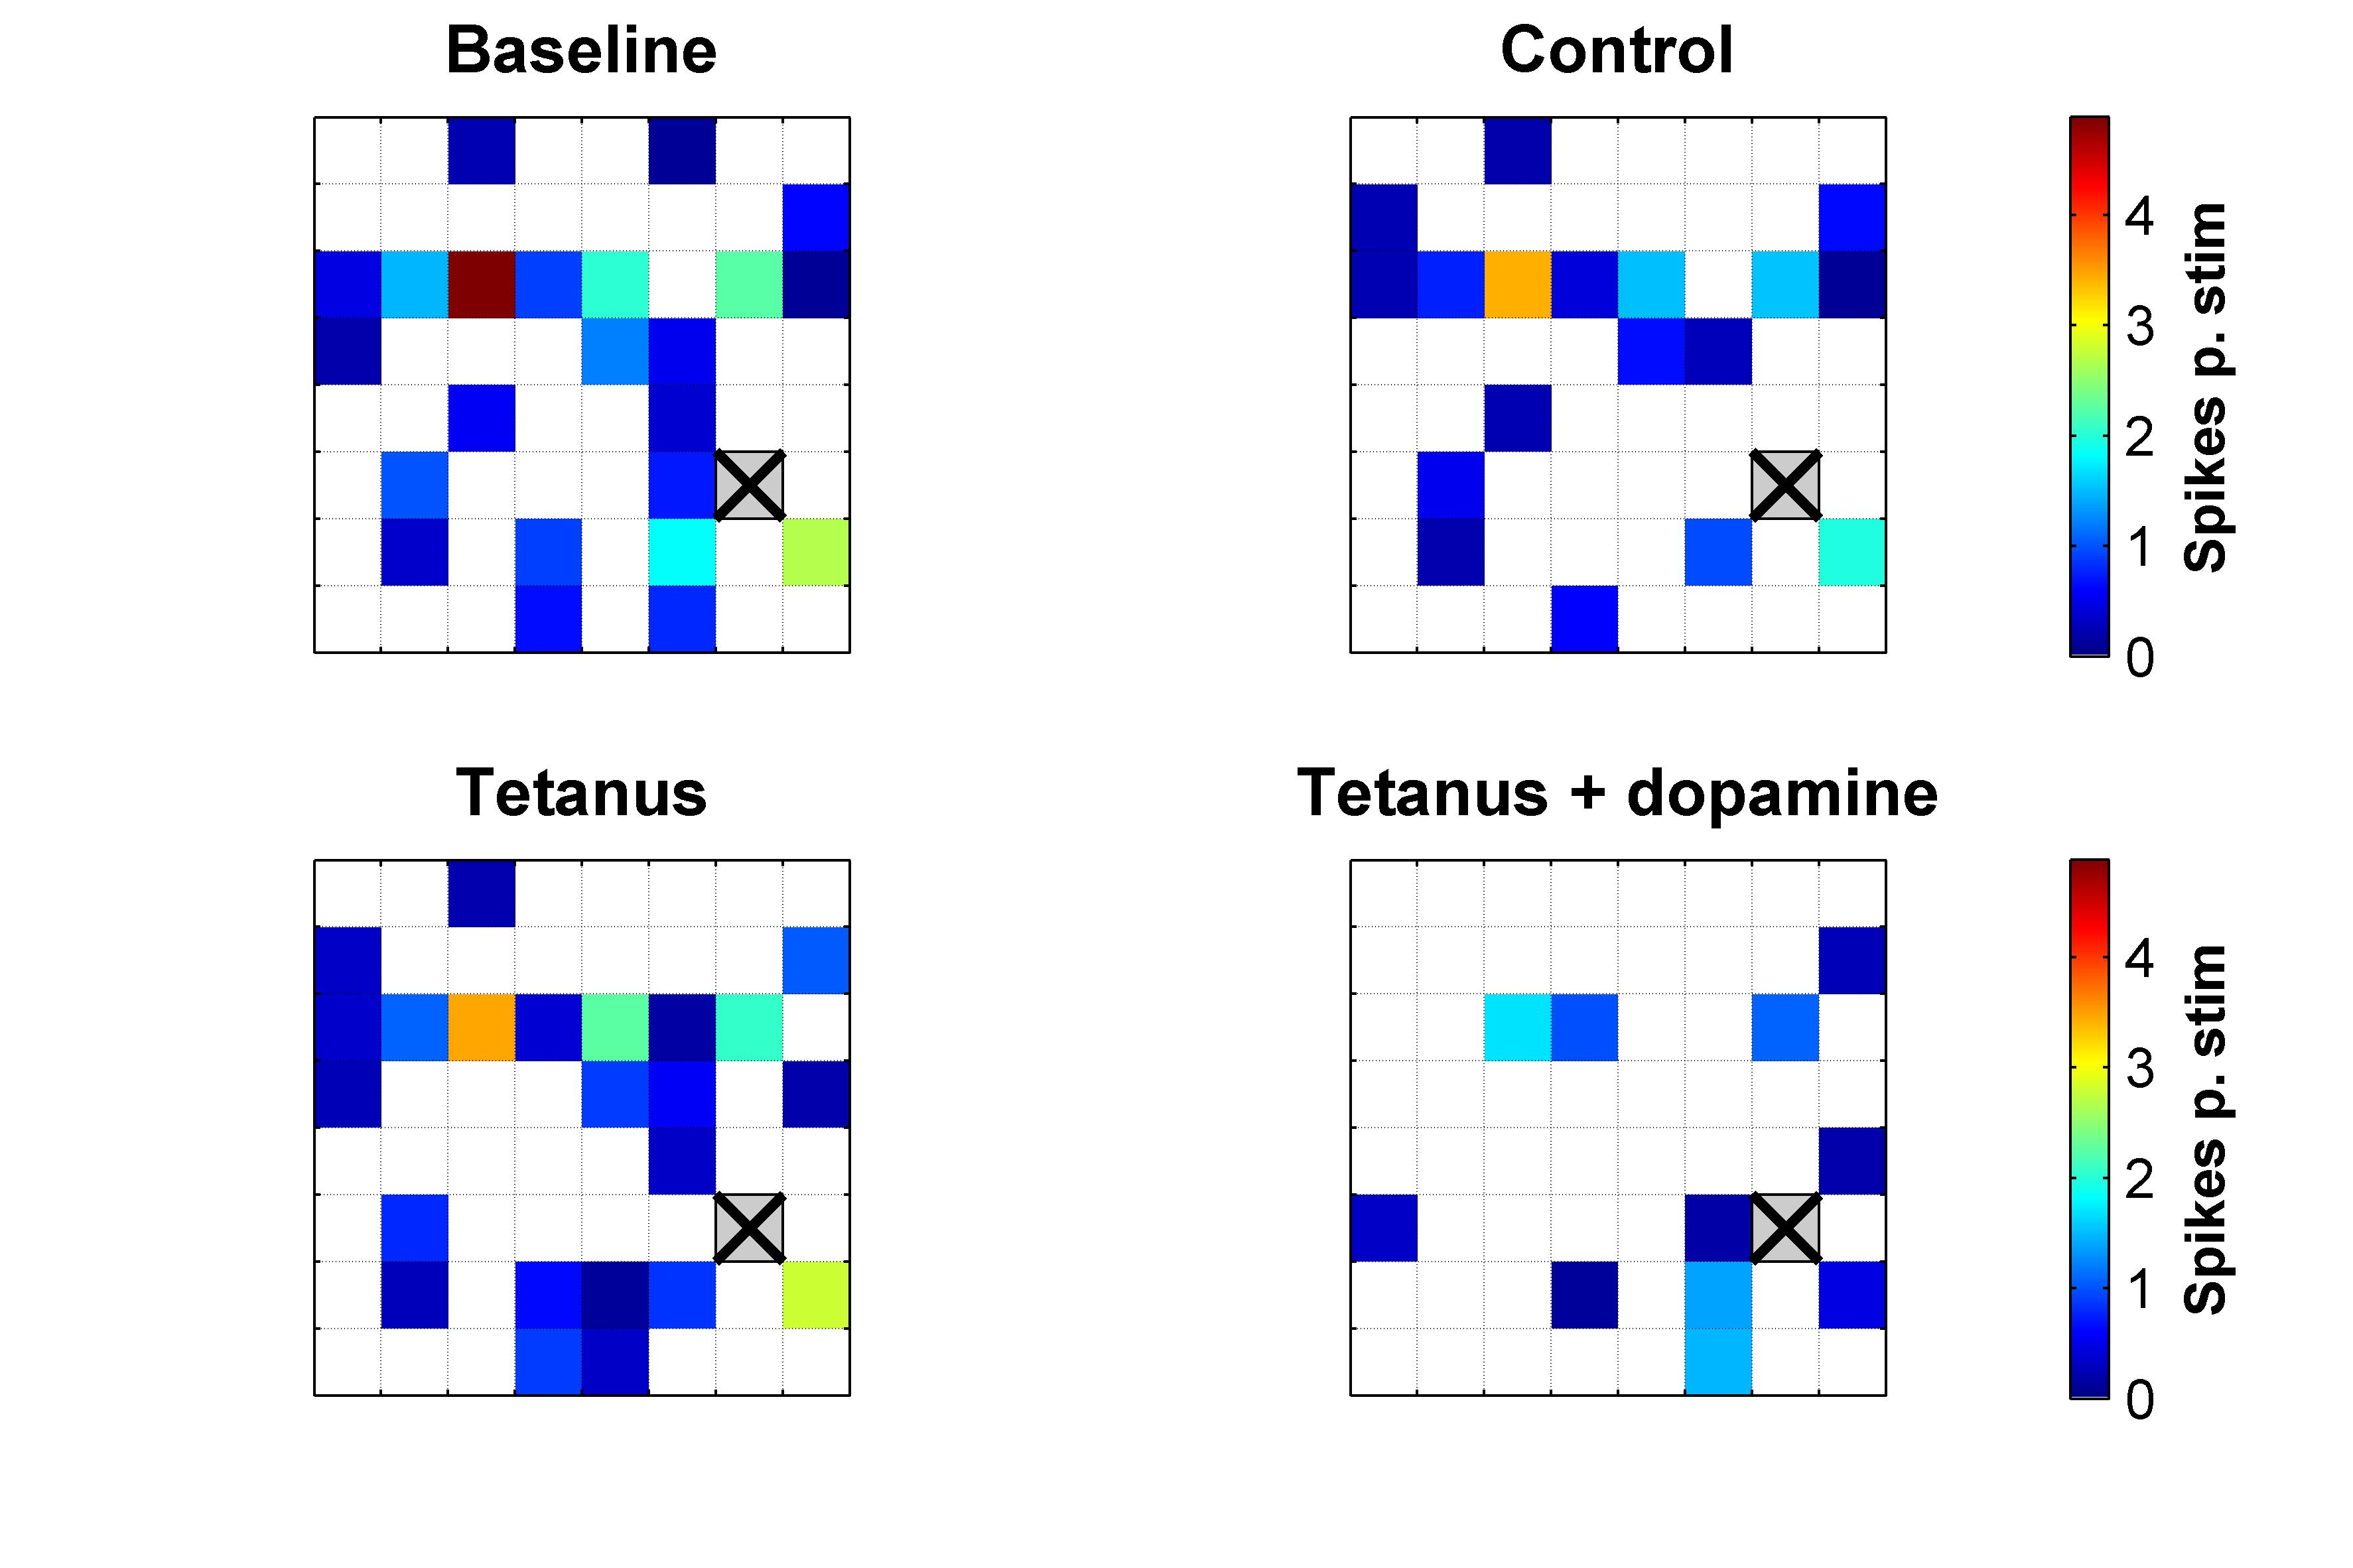
\includegraphics[width=15cm]{chapter3/figures/tetMapChange/tetMapChange.jpg}

            \caption[Example stimulation response maps for the combined dopamine and tetanus plasticity induction experiment]{\textbf{Tetanus combined with a dopamine pulse but not tetanus alone induces a reduction in the number of responsive channels.} Stimulation response maps of the same data presented in figure \ref{fig:activity:tetStimChange}.}
            \label{fig:activity:tetMapChange}
        \end{figure}


        \begin{figure}[!htb]
         \centering
         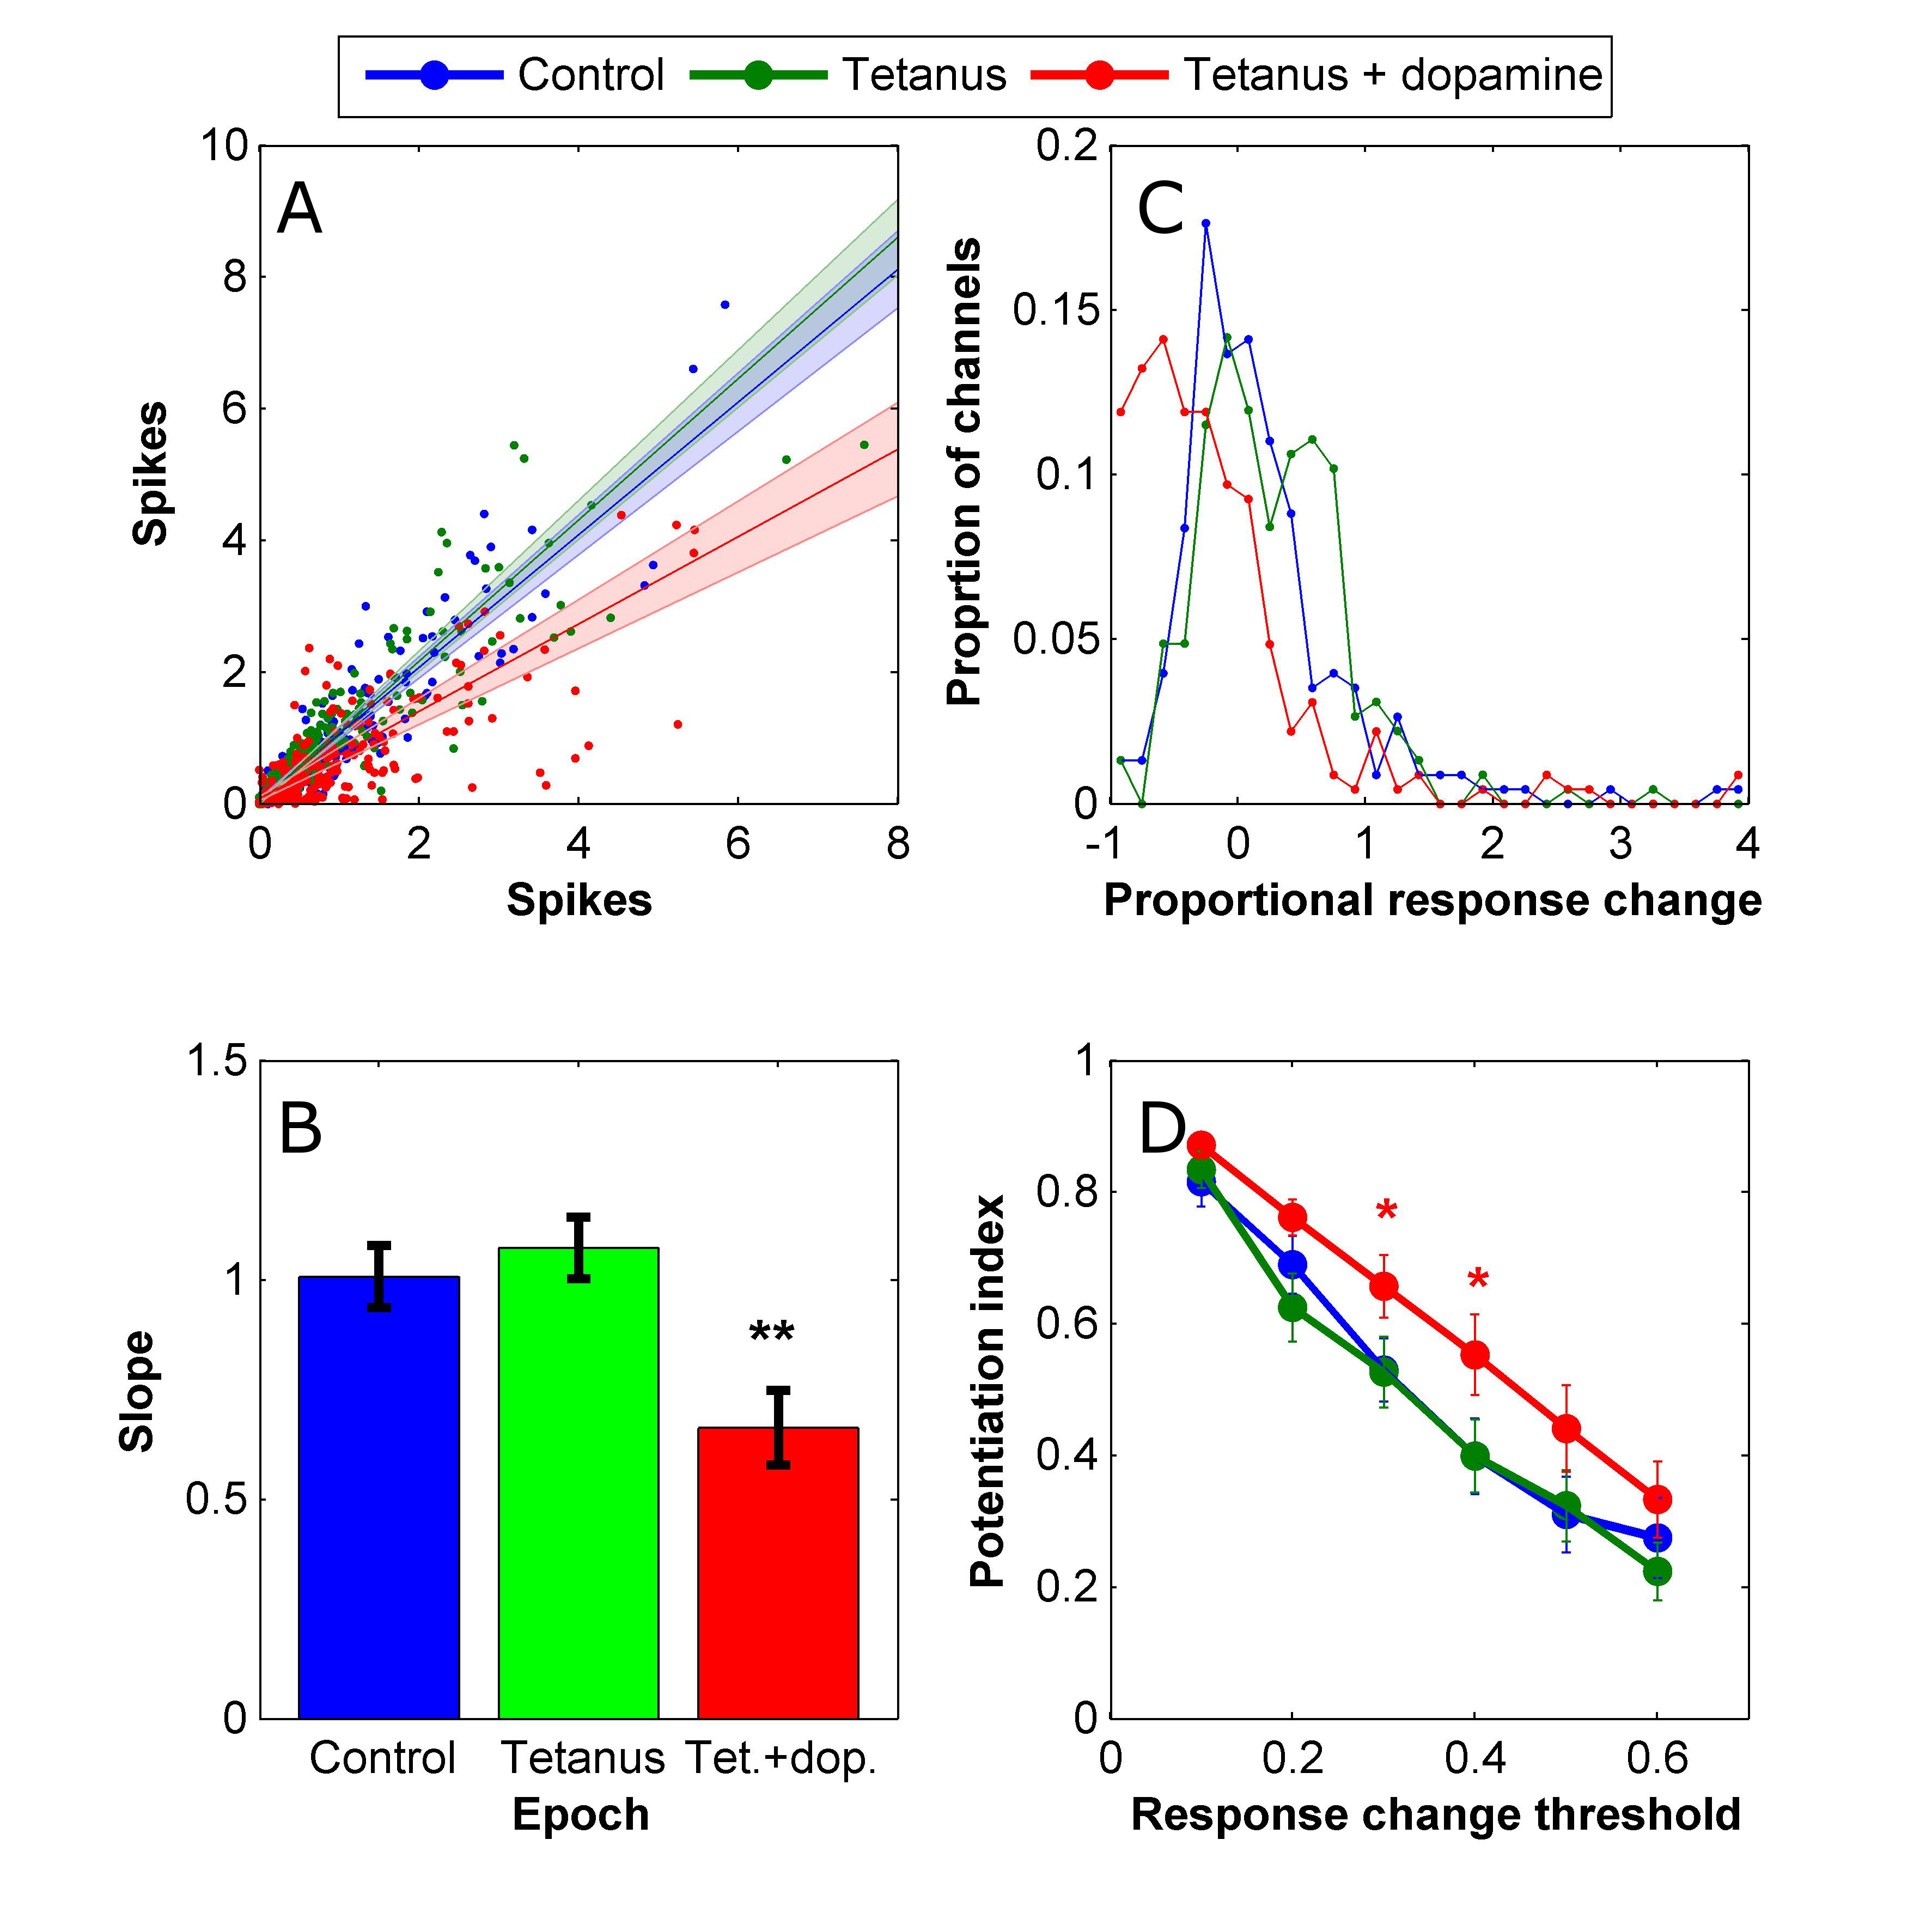
\includegraphics[width=15cm]{chapter3/figures/tetResChangeStats/tetResChangeStats.jpg}

         \caption[Statistics of changes to evoked responses in the combined dopamine and tetanus plasticity induction experiment]{\textbf{Tetanus combined with a dopamine pulse but not tetanus alone induces a depression of evoked responses.}(A) Scatter plot of pre induction vs. post induction channel responses for the 3 induction steps of our protocol. Data from all tested cultures and from all stimulating electrode are lumped. The analysis, however, considers each of these groups to be an independent data set and fits a line to each. Plotted lines and shaded areas visualize the mean and SEM of these line slopes. Data is based on 4 cultures \(\times\) 4 stimulating electrodes (n=16). (B) Comparison of fitted slopes from A. (C) Distributions of proportional changes induced in channel responses for the 3 induction steps of our protocol lumped as in A. For computation of potentiation index (PI) such distributions are generated for each data set. For each of these distributions the PI is the proportion of channels exceeding a threshold level of change. Finally, PI is computed for a range of thresholds and averaged over independent data sets (n=16 as in A). (D) Mean + SEM of potentiation index as a function of tested levels of change thresholds.}
         \label{fig:activity:tetResChange}
    \end{figure}


    Figure \ref{fig:activity:tetResChange} shows a statistical analysis of the plasticity induction experiments which closely follows the one performed in \cite{chiappalone2008network}. In essence, channel responses for each stimulating electrode were compared in a scatter plot of pre induction vs. post induction responses and a linear fit was computed (figure \ref{fig:activity:tetResChange} A-B). The slope for the 'associative tetanus' induction did not show a statistically significant difference from the one for the sham (control) induction (\(1.01\pm0.07\) vs. \(1.07\pm0.07\), 2-sided t-test, p=0.5). The slope for the induction performed in the presence of dopamine was significantly smaller, though (\(0.66\pm0.09\), 2-sided t-test, p=0.004), indicating a general depression in evoked responses (i.e., across all channels). The potentiation index analysis provided results to the same effect. This analysis is based on generating distributions of proportional changes to the channel responses before and after the induction (figure \ref{fig:activity:tetResChange} C). Potentiation index is a measure for comparing these distributions and is defined as the proportion of channels with absolute change exceeding a predefined threshold. By selecting the threshold correctly, a distinction between the distributions based on their width can be generated even if their mean is the same. In other words, this measure is designed to detect more subtle changes to the network activity that may include some of the channels experiencing large but antagonistic changes which cancel out when looking at the mean. In more common terms, one could say this is a variance or a second order measure. Since the appropriate threshold for making the distinction between the distributions is unknown, potentiation index is computed for several thresholds over the entire range of the data. It should be mentioned that the name 'potentiation index' is somewhat of a misnomer as it refers not to potentiation in the sense of strengthening but to absolute change. At any rate, applying this analysis to our plasticity induction data did not reveal any significant differences between the tetanus and control inductions. The tetanus induction in the presence of dopamine, on the other hand, showed a significantly higher potentiation using change thresholds of 0.3 and 0.4 (figure \ref{fig:activity:tetResChange} D, 1-sided t-test, p=0.034 and 0.039, respectively). This, however, is not surprising given that a general depression was observed in the preceding slopes analysis.






        \subsection{Examining changes in functional connectivity}
           Since the aforementioned analyses did not reveal any tetanus-only induced plasticity we decided to try a yet finer probing of the network activity. This is based on the functional connectivity (FC) analysis which was reported to capture plasticity in response to tetanus \cite{le2015repeated}. Mathematical details and examples for computation of functional connectivity are given in section \ref{sec:methods:FC}. In essence, the measure is based on locating peaks in the cross correlation function between channel pairs normalized to the number of spikes in the first channel. The size of the peak reflects the probability of recording a spike in the second channel following a spike in the first one at a time captured by the latency of the peak. This computation therefore results in 2 vectors, one holding peak sizes (also termed FC strengths) and the other peak latencies. Finally, differences in functional connectivity between recording epochs is measured as the Euclidian distance between the appropriate vector from the compared epochs. In our analysis we looked only at distances in the FC strengths vector because situations where the functional connectivity is lost completely (i.e., connection strength becomes 0) do not require special treatment. It has been claimed that this measure is more efficacious at detecting plasticity when computed over spontaneous activity \cite{le2015repeated} so we indeed used the spontaneous activity periods of recording in our protocol for its computation.

        \begin{figure}[!htb]
            \centering
            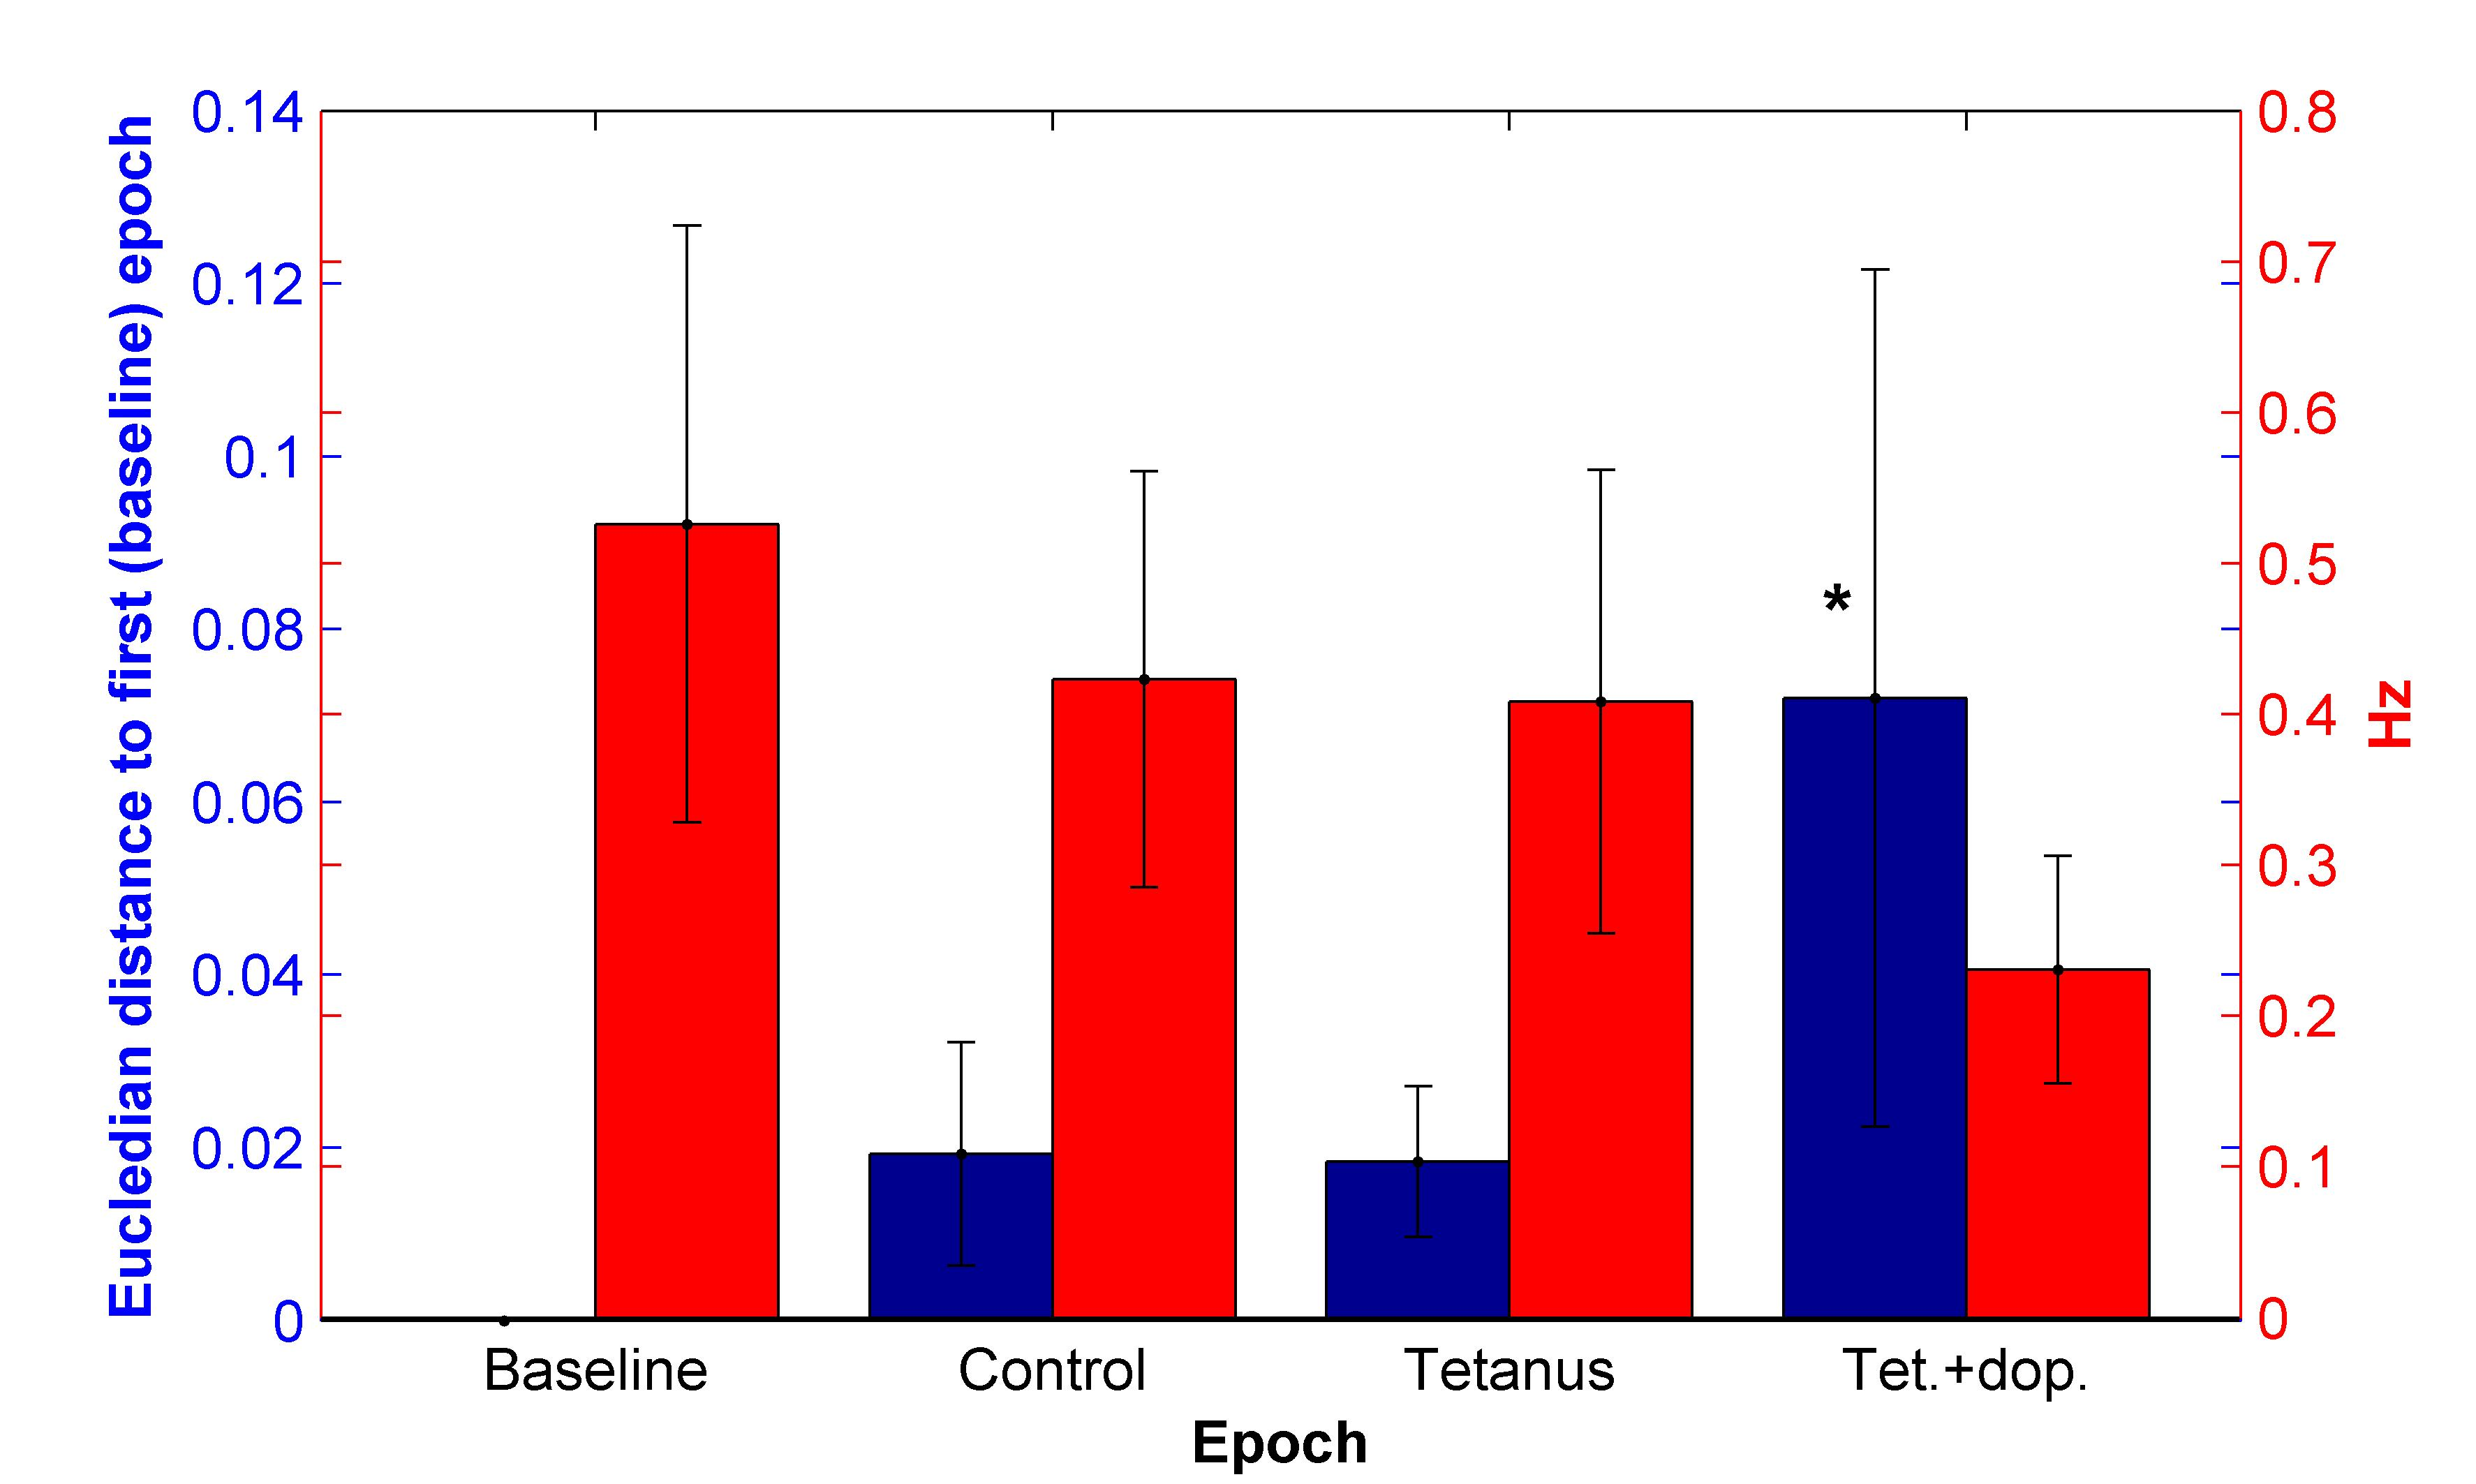
\includegraphics[width=15cm]{chapter3/figures/FCChangeStats/FCStats.jpg}

            \caption[Statistics of Change to functional connectivity and average unit firing rate in the combined dopamine and tetanus plasticity induction experiment]{\textbf{Tetanus combined with a dopamine pulse but not tetanus alone induces a change to functional connectivity as well as a decrease to spontaneous activity.} Blue bars: Euclidean distance of the functional connectivity strength vector from baseline following each induction epoch. Functional connectivity was computed based on the spontaneous activity period in each of the measurement epochs. Functional connectivity computation requires a minimum number of spikes in each of the analyzed channel pairs to generate a meaningful cross correlation function estimation (see section \ref{sec:methods:FC}) so only a subset of the possible recording channel pairs normally participate in the analysis. One of the cultures participating the the plasticity induction had to be removed as it had no channel pairs complying with the above criteria. Thus the shown data are based on n=3 cultures with 33, 10 and 179 computable functional connectivity pairs. Red bars: Mean channel firing rates in the same spontaneous activity measurement periods. This data are based on all n=4 participating cultures.}
            \label{fig:activity:tetFCChange}
        \end{figure}

           Figure \ref{fig:activity:tetFCChange} shows the changes to the functional connectivity over the different experimental protocols (measured as Euclidian distance from the baseline epoch) as well as the mean channel firing rate. The results show that the tetanus induction itself did not generate a change to the functional connectivity beyond naturally occurring fluctuations that were already observed after the control induction. A larger change was observed following the tetanus induction in the presence of dopamine which proved to be statistically significant (1-sided t-test, p=0.026). However, this change was also accompanied by a strong decrease in the mean channel firing rate which, for this data set, proved to be significant with only 90\% confidence (1-sided t-test, p=0.097). In light of this change to the averaged culture activity, the observed shift in the functional connectivity measure should be taken with a grain of salt as it was designed to reflect subtle changes to the underlying culture structure in conditions where first order statistics (such as mean firing rate) are stable.


  \subsection{Comparison between mouse and rat cultures}
    \label{sec:activity:mouseRatComp}
    As mentioned in the beginning of section \ref{sec:activity:spontActivity}, the mouse cultures posed a difficulty of a high culturing failure rate which, together with the fact that they exhibited delayed electrophysiological development raised concerns regarding their utility and ease of use. We therefore decided that, following the study performed in this chapter, rat based preparations would be used for the remainder of the Ph.D work. Here we outline a brief pilot study to compare our rat based preparations with the mouse based ones and assert that the former shows an electrophysiological profile in par with the literature. In order to compare the functional development of mouse based and rat based cultures we recorded spontaneous activity from a set of rat cultures, prepared using a protocol identical to the mouse ones.

       \begin{figure}[!htb]
            \centering
            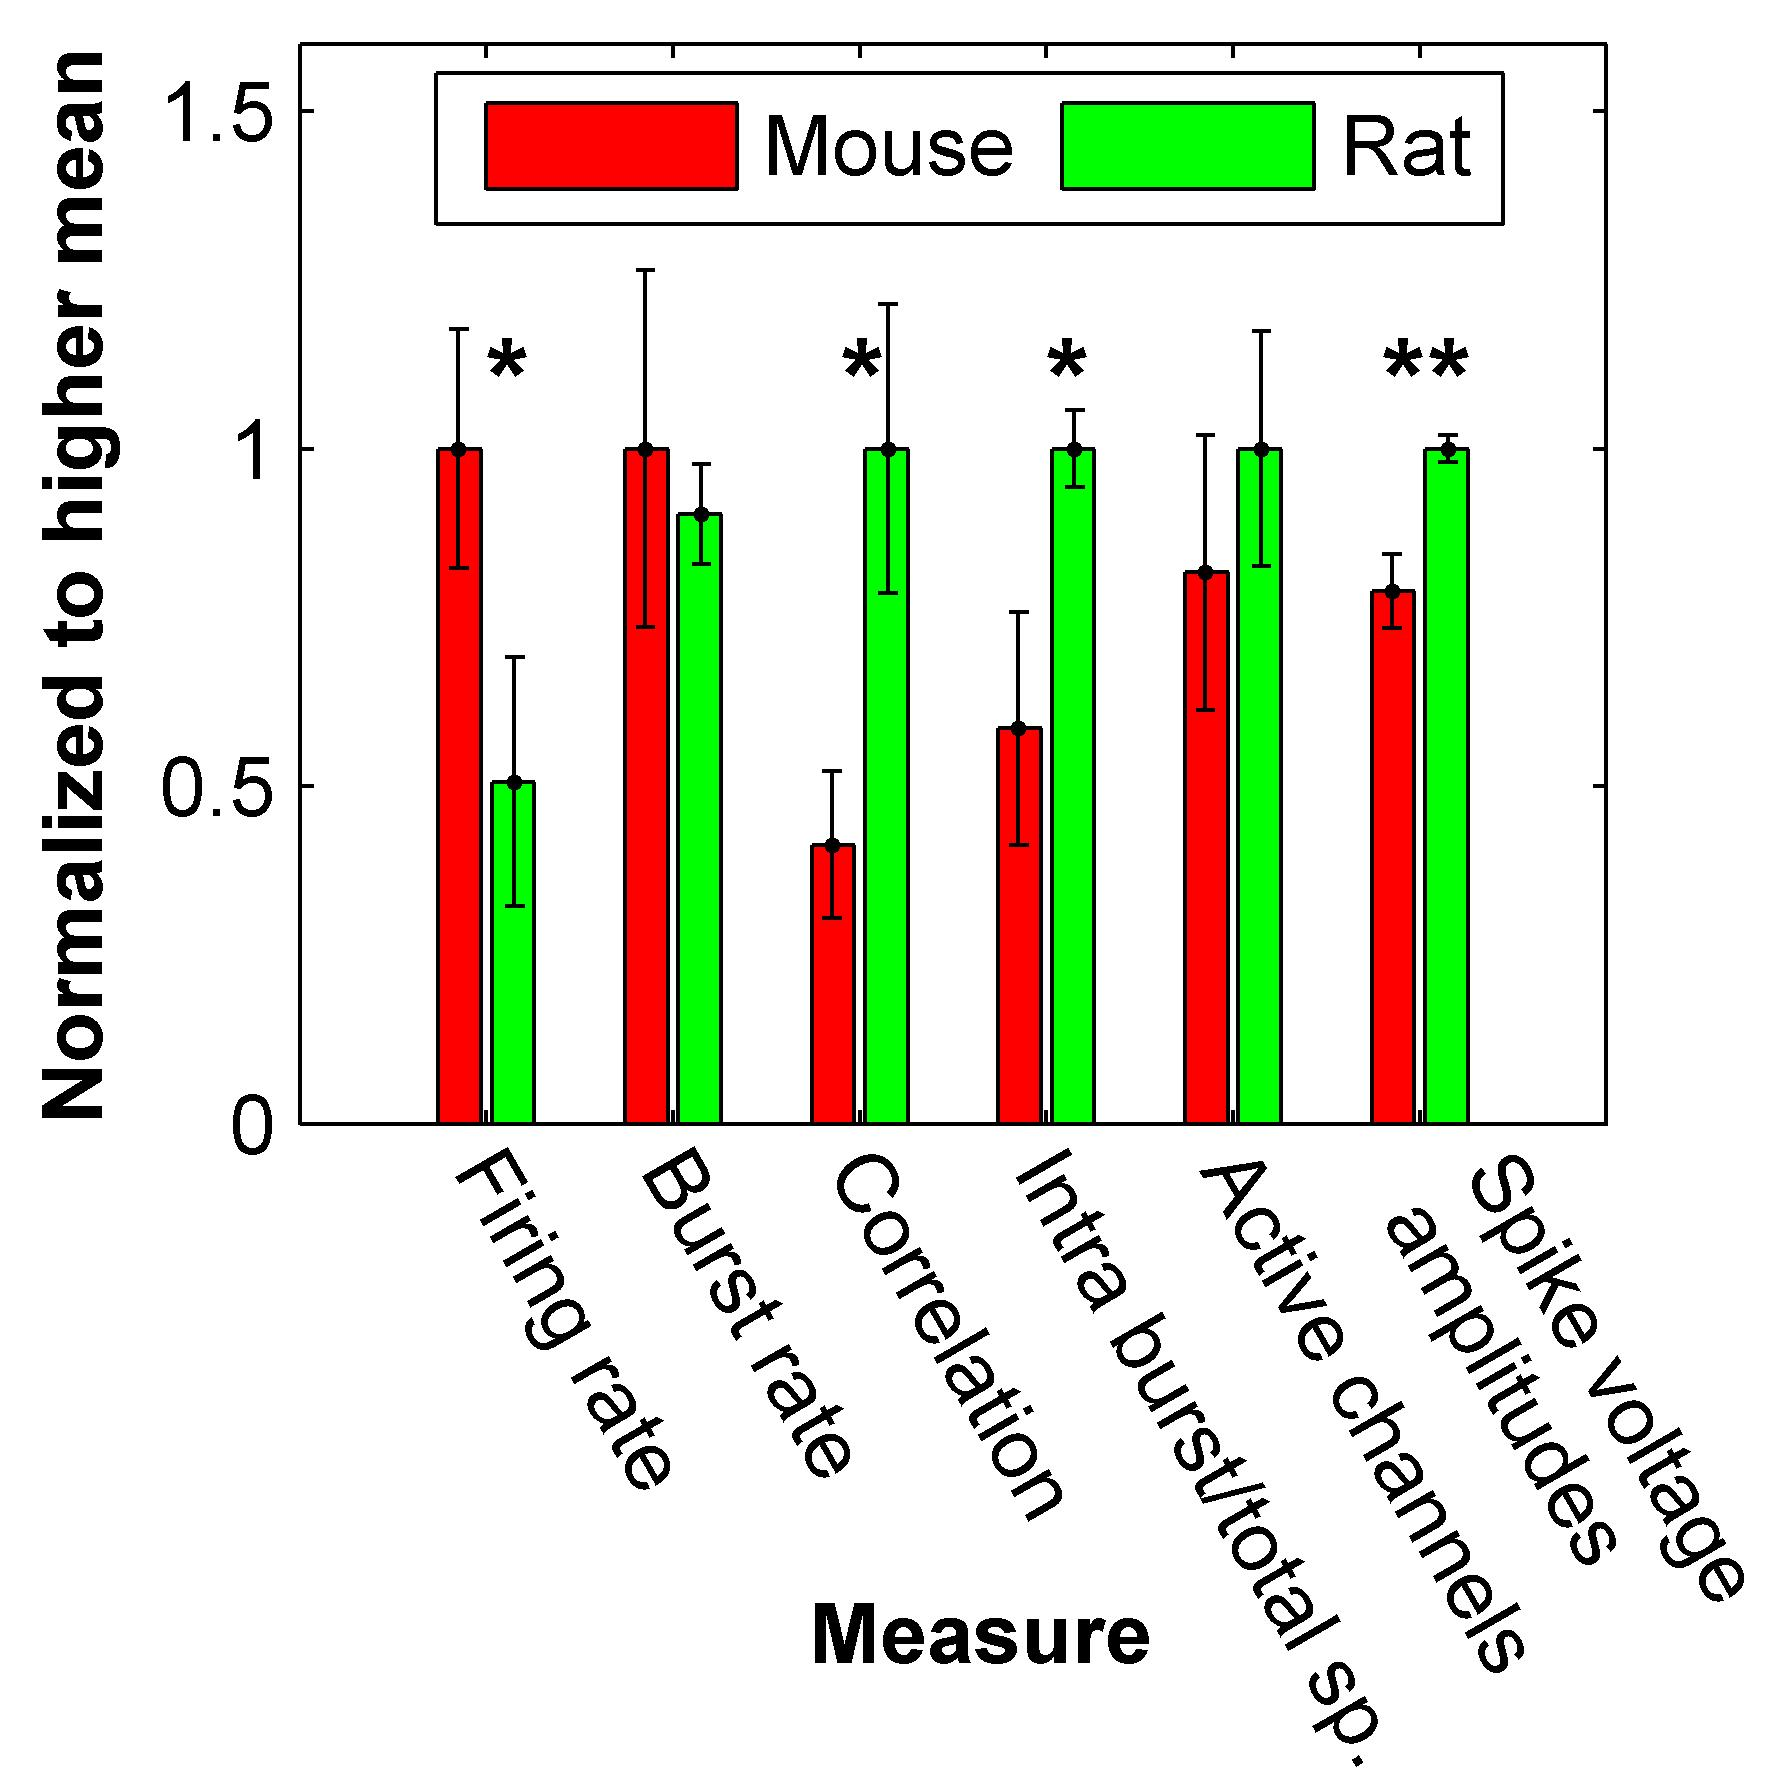
\includegraphics[width=7.5cm]{chapter3/figures/mouseRatComp/ratMouseComp.jpg}

            \caption[Comparison between spontaneous activity in mouse and rat based cultures]{\textbf{Rat cultures show increased correlation as compared to rat cultures at the same age.} Six measures are considered and are normalized to whatever mean is higher amongst the two compared groups. *, ** indicate statistical significance of the difference between the groups at levels of confidence of 95\% and 99\%, respectively. Mouse statistics are based on n=5 cultures and rat statistics on n=4 cultures. Culture ages at the time of recording were selected so that both groups had the same mean age of 19.5 days \textit{in vitro} (range \(15-23\) DIV for rat and \(18-20\) DIV for mouse).}
            \label{fig:activity:mouseRatComparison}
       \end{figure}

    Figure \ref{fig:activity:mouseRatComparison} shows a comparison between rat based and mouse based cultures at the same age \textit{in vitro} for several activity and synchronicity measures introduced earlier. A particularly pronounced difference was observed in the closely related measures of correlation and ratio of intra-burst to total activity both of which showed a significantly higher values in the rat cultures (1-sided unbalanced t-test, p=0.017 and 0.039, respectively). These differences demonstrate that mouse cultures exhibited more uncorrelated activity as compared with their rat counterparts. This reiterates the observation discussed in the previous section that the mouse cultures show delayed synaptic development.

    Another observed difference is that the mouse cultures showed a significantly higher average unit firing rate (one sided unbalanced t-test, p=0.048). This result could be another manifestation of the rat neurons being more attuned to the synaptic drive from the network but is harder to interpret. In any case, the mean values for both preparations types (\(1 Hz\) and \(0.5 Hz\) for mouse and rat, respectively) are within the literature range (\(0.4-1.5 Hz\)).

    Both preparations showed a nearly identical burst rate of about 15 minute\textsuperscript{-1}. The burst rate measure is different to the correlation and activity ratio measures in that it counts synchronized events but is indifferent to activity outside such events. This in contrast to the correlation and intra-burst to total spikes ratio measures which are sensitive to activity both inside and outside the bursts. The fact that the reduced synaptic coupling in mouse cultures does not affect the burst rate suggests that the this measure is strongly related to the general excitability and not just to the synaptic development.

    Finally, the spike amplitudes measure shows the mean of peak voltage in the recorded extracellular spike waveforms across all mouse and rat recordings (see section \ref{sec:methods:MEARecording} for example waveforms). Surprisingly, we found a significant reduction in peak voltage for the recording from mouse preparations as compared to the rat preparations. This indicates that the two types of neurons are different in their excitability properties and that, possibly, mouse neurons express a lower density of voltage dependent ion channels.

    In summary, the comparison confirmed that the mouse cultures are delayed in synaptic maturation as compared to rat cultures and thereby display reduced correlations at the same age \textit{in vitro}. As far as these results can corroborate, our rat based preparations present all the features and developmental time course that have been described in literature and will therefore will be selected for the work carried out in the following chapters.


    \section{Chapter conclusion}
    The main purpose of this chapter was to establish the standard neuronal culture on MEAs model system together with the accompanied Matlab analysis and show that the cultures are healthy and exhibit the diverse electrophysiological characteristics which have made them a successful neuroscience model system. Indeed distinct stages of development of network activity were clearly observed. These consisted of initial uncorrelated but widespread firing patterns corresponding to neuronal maturation followed by an increase in correlations and rate of synchronized events which indicate that the synapses are maturing. Further examination of the data revealed evidence for other neurobiological processes that have been described in culture. These included homeostasis of activity rates, existence of strongly intra-connected subnetworks and a gradual temporal narrowing of the synchronized events which has been attributed to a delayed maturation of the GABA neurotransmission system as compared to the glutamatergic one. These processes have not been studied here in depth but are taken as evidence that our cultures are healthy and in par with the literature. It is important to note that these observations have been made on mouse cultures which have been seldom used in the MEA context. The provided data thus establish their usability even though certain difficulties were also reported which made us eventually switch to using rat cultures.

    The final undertaking of this chapter was to explore a protocol for phasic application of dopamine using manual pipetting. We modified a common plasticity protocol to include a step where dopamine is applied exclusively during the tetanus induction step (through manual pipetting and subsequent washing). Without any dopamine, we were not able to induce a change in the culture activity, despite reports to the contrary in the paper from which the protocol was adapted. This should not come as a surprise as the literature is controversial in this regard and should just serve as a demonstration that further work is required for these systems to serve as a useful model of plasticity. Following a tetanus induction which was performed in the presence of dopamine a significant depression was observed in the evoked responses which were measured up to an hour following the induction. The spontaneous activity was also depressed but to a lesser extent. On one hand this could demonstrate an enablement of LTD by the dopamine. The fact that this effect is present after the dopamine had been removed strengthens the possibility that this is a plasticity effect rather than a result of direct interaction of the cells with the agonist. Indeed a similar experiment had been performed in cortical slices and produced very similar results \cite{otani1998dopamine}. On the other hand, it is also known that in neuronal culture the mere action of media replacement drastically reduces activity (this  will be made very clear by the results of chapter \ref{chap:activityAndFlow}), an effect the could last several hours. Additionally, the presence of dopamine itself is known to have an inhibitory effect in the cortex regardless of plasticity \cite{gu2002neuromodulatory,gonzalez2001dopamine} and it is hard to rule out the option that a small concentration of the agonist is still present after the washing step and contributing to the observed effect. Under the constraints of the current bath application methods, it is impossible to run a dopamine pulse without these impinging effects. Undoubtedly we could quantify them by using a set of control experiments but we cannot eliminate them.

    To summarize, these dopamine pulsing results are promising in that they suggest a potential for dopamine to enable plastic behaviour in culture. However, this notion wasn't fully proven due to uncertainty about the effects of media replacement and of temporary interaction of dopamine with the neurons. This highlights the need for a precise solution exchange system whereby dopamine can be applied with high spatio-temporal precision and without change to other extracellular ingredients which could interfere with the activity. Such a system would allow interrogation into the fine temporal details of the phasic dopamine and volume transmission processes in general far beyond what was demonstrated in the above-described work. The following chapters in this Ph.D thesis will describe the development and establishment of a microfluidic based rapid solution exchange system where the drug delivery is rapid, precise and decoupled from other changes to the extracellular chemistry.
